%volby: 
% male × female
% czech × english (zatím funguje jen czech)
% a studijní program / obor 
% is_bc (nejvíc odladěno)
% api_bc
% api_ing
% edu_bc
% edu_ing

\documentclass[male,czech,api_ing]{thesis}
\usepackage{ifthen}

\usepackage{amsmath,amssymb}
\usepackage{graphics}
\usepackage{color}
\usepackage{array}
\usepackage{longtable}
\usepackage{afterpage}
\usepackage{microtype}  % přesnější typografie
\usepackage{xcolor}
\usepackage{graphicx}

% Algorithms
\usepackage{algorithm}
\usepackage{algpseudocode}
\makeatletter
\renewcommand{\ALG@name}{Algoritmus}
\makeatother

\graphicspath{ {./images/} }

\usepackage{float}

% workaround for imcompatibility of czech babel and biblatex

\iftutex
\else
\usepackage{etoolbox}
\makeatletter
\newcommand\my@hyphen{-}
\newcommand\my@apostroph{'}
\patchcmd\select@language{-}{\my@hyphen }{}{}
\patchcmd\select@language{'}{\my@apostroph }{}{}
\makeatother
\fi

% fonty lze měnit (detaily viz sekce fonty)
\iftutex
	\usepackage{fontspec}  % nastavení fontů pro LuaLaTeX a XeLaTeX
	\setmainfont{Libertinus Serif}
	\setsansfont{Libertinus Sans}
	\setmonofont[Scale=MatchLowercase]{Libertinus Mono}
	\usepackage{unicode-math}
	\setmathfont{Libertinus Math}
\else
	\usepackage[utf8]{inputenc} % nastavení pro PDF LaTeX
	\usepackage[T1]{fontenc}
	\usepackage{libertinus}
	\renewcommand{\ttdefault}{pxtt}
\fi

\usepackage[style=iso-numeric,shortnumeration=true]{biblatex}
\addbibresource{thesis.bib}

\usepackage{csquotes} % uvozovky

% sazba ukázek kódu 

\usepackage{listings}
\renewcommand{\lstlistingname}{Ukázka kódu}

\lstdefinestyle{DOS}
{
    basicstyle=\scriptsize\color{black}\ttfamily,
    breaklines=true,
}

\definecolor{codegreen}{rgb}{0,0.6,0}
\definecolor{codegray}{rgb}{0.5,0.5,0.5}
\definecolor{codepurple}{rgb}{0.58,0,0.82}
\definecolor{backcolour}{rgb}{0.95,0.95,0.92}

\lstset{
    language=Python,
    backgroundcolor=\color{backcolour},
    keywordstyle=\color{magenta},
    numberstyle=\tiny\color{codegray},
    stringstyle=\color{codepurple},
    basicstyle=\small\ttfamily,
    showspaces=false, 
    showstringspaces=false, 
    showtabs=false,
    frame=tb, 
    tabsize=3, 
    breaklines=true,
    breakatwhitespace=false, 
    numbers=left,
    extendedchars=true,
    inputencoding=utf8,
    escapeinside={(*}{*)},
}

% sazba matematických výrazů
% \newenvironment{conditions}[1][kde:]
%     {#1 \begin{tabular}[t]{>{$}l<{$} @{${}={}$} l}}
%     {\end{tabular}\\[\belowdisplayskip]}

\newenvironment{conditions}[1][kde:]
    {#1 \begin{tabular}[t]{>{$}l<{$} @{${}={}$} >{\raggedright\arraybackslash}p{10cm}}}
    {\end{tabular}}

% barevné zvýraznění textů, které je nutno nahradit
\newcommand{\ZT}[1]{\colorbox{yellow}{\color{red}{#1}}}


% TOTO JE POTŘEBA ZMĚNIT !!!!!!
\newcommand{\nazevcz}{Vliv předzpracování obrazu a augmentace dat na segmentaci rentgenových snímků}        % zde VYPLŇTE český název práce (přesně podle zadání!)
\newcommand{\nazeven}{Impact of image preprocessing and data augmentation on segmentation of X-ray images}     % zde VYPLŇTE anglický název práce (přesně podle zadání!)
\newcommand{\autor}{Bc. Milan Gittler}           % zde VYPLŇTE své jméno a příjmení
\newcommand{\rok}{\the\year}                
\newcommand{\vedouci}{RNDr. Jiří Škvára, Ph.D.}         
% zde VYPLŇTE jméno a příjmení vedoucího práce, včetně titulů
\newcommand{\vedouciDAT}{RNDr. Jiřímu Škvárovi, Ph.D.}   
% zde VYPLŇTE jméno a příjmení vedoucího práce, včetně titulů ve třetím pádě
                                                           
% zvětšuje o 23% vertikální okraje v tabulkách
\renewcommand{\arraystretch}{1.23}

% nastavení pro záhlaví (co nelze udělat v cls souboru)
\renewcommand{\chaptermark}[1]{\markboth{\arabic{chapter}. #1}{}}
\pagestyle{fancy}

% nastavení odkazů
\usepackage{url} % formátování URL, příkaz \url
\usepackage{varioref} % lepší interní odkazy na obrázky, apod. příkaz \vref
\usepackage[unicode=true,pdfusetitle,
 bookmarks=true,
 breaklinks=false,pdfborder={0 0 1},backref=false,colorlinks=false]{hyperref} % hypertextové odkazy v PDF

\counterwithin{figure}{section}

\renewcommand{\listfigurename}{Seznam obrázků}
\renewcommand{\lstlistlistingname}{Sazba zdrojových kódů}

\begin{document}
\afterpage{\null\newpage}
\thispagestyle{empty}
\begin{center}
{
\LARGE
\univerzita\\[16pt]
\fakulta
}

\vspace{2cm}
\resizebox{8.42cm}{!}{%
\ifthenelse{\boolean{czech}}
{
\includegraphics{Prilohy/Logo/LOGO_PRF_CZ_RGB_standard.jpg}}
{
\includegraphics{Prilohy/Logo/LOGO_PRF_EN_RGB_standard.jpg}}}

\vspace{2cm}
{
\Huge\sffamily
\nazevcz\par
\vspace{0.6cm}
\Large\scshape \ifthenelse{\boolean{bc}}{bakalářská}{diplomová} práce
}
\end{center} 
 
\vfill
{
\large
\begin{tabular}{>{\bfseries}rl}
    Vypracoval: 	& \autor\\
    Vedoucí práce: 	& \vedouci\\
&\\
Studijní program:       & \program\\
% \ifthenelse{\boolean{api}}{Studijní obor:          & \obor\\}{}
\end{tabular} 
}
\vspace{1.5cm}
\begin{center}
  \Large\scshape   Ústí nad Labem \rok
\end{center}

\cleardoublepage
\thispagestyle{empty}
\pagecolor{yellow}
{\Large Namísto žlutých stránek vložte digitálně podepsané zadání kvalifikační práce poskytnuté vedoucím katedry.\\\
Zadání musí zaujímat právě dvě strany.
}

Zadání je nutno vložit jako PDF pomocí některého nástroje, který umožňuje editaci dokumentů (se zachováním
elektronického podpisu).

V Linuxe lze například použít příkaz \texttt{pdftk}.

\clearpage
\thispagestyle{empty}

\afterpage{\nopagecolor}
~
\clearpage

\thispagestyle{empty} 
{\bfseries Prohlášení}

\vspace{0.5cm}
Prohlašuji, že jsem tuto \ifthenelse{\boolean{bc}}{bakalářskou}{diplomovou} práci vypracoval\ifthenelse{\boolean{feminum}}{a}{}
samostatně a použil\ifthenelse{\boolean{feminum}}{a}{}
jen pramenů, které cituji a uvádím v přiloženém seznamu literatury.

\vspace{0.5em}

Byl\ifthenelse{\boolean{feminum}}{a}{} jsem seznámen\ifthenelse{\boolean{feminum}}{a}{} 
s tím, že se na moji práci vztahují práva a povinnosti vyplývající ze
zákona c. 121/2000 Sb., ve znění zákona c. 81/2005 Sb., autorský zákon, zejména se
skutečností, že Univerzita Jana Evangelisty Purkyně v Ústí nad Labem má právo na uzavření
licenční smlouvy o užití této práce jako školního díla podle § 60 odst. 1 autorského zákona, a
s tím, že pokud dojde k užití této práce mnou nebo bude poskytnuta licence o užití jinému
subjektu, je Univerzita Jana Evangelisty Purkyně v Ústí nad Labem oprávněna ode mne
požadovat přiměřený příspěvek na úhradu nákladu, které na vytvoření díla vynaložila, a to
podle okolností až do jejich skutečné výše.

\vspace{2em}

V Ústí nad Labem dne \today   \hfill Podpis: \makebox[4cm][s]{\dotfill}

\cleardoublepage
\thispagestyle{empty}
~
\vfill

\begin{flushright}
    Děkuji vedoucímu práce {\vedouciDAT}\\ 
    za neocenitelné rady a pomoc při tvorbě diplomové práce.
\end{flushright}

\cleardoublepage

\textsc{\nazevcz}

\textbf{Abstrakt:}

Hlavním cílem této diplomové práce je ohodnotit vliv předzpracování obrazu a augmentace dat na segmentaci rentgenových snímků. Čtenář je nejdříve seznámen se standardními algoritmy pro vylepšení obrazu a redukci šumu. Dále jsou v práci představeny neuronové sítě a základní principy fungování společně s implementací vybraných architektur pro redukci šumu. V neposlední řadě jsou popsané metody aplikovány na rentgenové snímky dvou datových sad a je měřena výkonnost a efektivita modelů pro segmentaci obrazu v závislosti na předchozím zpracování dat.

\textbf{Klíčová slova:} Předzpracování obrazu, Neuronové sítě, Segmentace obrazu, U-Net

\bigskip


\textsc{\nazeven}

\textbf{Abstract:}

The main objective of this thesis is to measure the impact of image preprocessing and data augmentation on the segmentation of X-ray images. The reader is first introduced to standard algorithms for image enhancement and noise reduction. Furthermore, neural networks and the basic principles of their operation are presented, along with the implementation of selected architectures for noise reduction. Finally, the described methods are applied to X-ray images from two datasets, and the performance and efficiency of the image segmentation models are measured depending on the prior data processing.

\textbf{Keywords:} Image preprocessing, Neural networks, Image segmentation, U-Net

\tableofcontents

\addchap{Úvod}
Segmentace lékařských snímků je klíčovou oblastí, která výrazně ovlivňuje kvalitu a efektivitu diagnostických procesů. V dnešní době, kdy je stále více kladen důraz na rychlou a přesnou diagnózu, se využití automatizovaných metod stává nezbytnou součástí při zpracování medicínských dat. Tradiční metody segmentace, založené na ručním označování, jsou časově velmi náročné a mohou být náchylné na tvorbu chyb. S rozvojem umělé inteligence a hlubokého učení se otevírá možnost využití pokročilých algoritmů, které mohou tento proces výrazně urychlit a zefektivnit. Tyto metody jsou ovšem velmi často aplikovány na data, která nemusí být ve vysoké kvalitě či mohou být určitým stylem degradována, a proto může být pro algoritmy obtížné vykonat zadanou úlohu správně.

Hlavním cílem této práce bude prozkoumat, jakým způsobem může předzpracování obrazu a augmentace dat ovlivnit segmentaci rentgenových snímků. Vzhledem k různorodosti a složitosti lékařských dat je předzpracování klíčovým krokem, který může významně ovlivnit výkonnost použitých modelů. Někdy bývá problémem nedostatečné množství dat nebo jejich pořízení je náročné. Z tohoto důvodu je důležité prozkoumat vliv augmentace dat, která umožňuje rozšířit datovou sadu a zlepšit tak podmínky pro učení neuronových sítí.

Práce bude strukturována dvou hlavních částí. V úvodní části budou představeny nejčastěji používané algoritmy pro vylepšení obrazu. Dále budou podrobně popsány vybrané metody, zaměřující se na redukci šumu v obraze. Informace o metodách umožní čtenáři pochopit princip fungování vybraných algoritmů, včetně způsobu jejich použití, výhod a nedostatků. Následně bude ukázán stručný přehled neuronových sítí, zejména konvolučních, zaměřených na zpracování obrazu a budou definovány hlavní komponenty, ze kterých se sítě skládají.

Druhá část práce se zaměří na představení a analýzu datových sad, na implementaci a aplikaci popsaných metod a také na návrh architektur neuronových sítí pro redukci šumu ve snímcích. Datové sady budou podrobeny různým typům šumu, aby bylo možné simulovat scénáře z reálného prostředí, se kterými se modely mohou v praxi setkat. Závěrečná část bude věnována měření vlivu předzpracování obrazu a augmentace dat na segmentaci rentgenových snímků pomocí modelů neuronové sítě U-Net. Budou provedeny experimenty s různými konfiguracemi, aby bylo možné zjistit, jak předzpracování ovlivňuje výkon segmentačních modelů. Implementační část práce bude dostupná na následujícím odkaze \url{https://github.com/Cemonix/Impact-of-Preprocessing}, kde lze najít podrobnosti o použitých metodách a dosažených výsledcích.

\chapter{Přehled metod předzpracování obrazu}
Tato kapitola se zabývá představením klíčových metod předzpracování obrazu, které hrají zásadní roli v procesu analýzy a zpracování rentgenových snímků. Předzpracování obrazu představuje kritický krok v řadě aplikací strojového učení a počítačového vidění, neboť ovlivňuje kvalitu a efektivitu následné analýzy. Metody předzpracování obrazu mohou výrazně zlepšit kvalitu dat a zvýšit přesnost detekce objektů, segmentace obrazu či klasifikace. Specifický výběr těchto technik je klíčový pro zjištění přesnosti a efektivity moderních metod počítačového vidění, včetně strojového učení a hlubokého učení, které jsou stále častěji aplikovány na širokou škálu problémů v oblasti zpracování obrazu. Zejména v kontextu rentgenových snímků může předzpracování pomoci překonat některé běžné výzvy, jako je nízký kontrast, šum, nebo artefakty, které mohou snížit kvalitu obrazu a tím ovlivnit diagnózu nebo automatickou analýzu.\cite{ImportanceOfImageProcessing}

\section{Klasické metody předzpracování obrazu}
Následující sekce se zabývá představením klasických metod a technik, které jsou využívány pro úpravu a zlepšení kvality obrazových dat před jejich dalším zpracováním. Budeme se tedy věnovat různým přístupům filtrace obrazu, metodám redukce šumu či zaostření obrazu, které jsou fundamentální pro analýzu a interpretaci obrazových dat. Přestože se jedná o metody, které mohou být považovány za základní, jejich správná aplikace a kombinace mohou výrazně zlepšit výslednou kvalitu obrazu a přispět k efektivnějšímu rozpoznávání vzorů a objektů v obrazových datech. Podrobně prozkoumáme každou z těchto metod, přičemž budeme klást důraz na jejich význam pro přípravu dat k dalšímu zpracování.

\subsection{Vylepšení obrazu}
Vylepšení obrazu je klíčovou technikou v předzpracování obrazu, zaměřenou na zlepšení vizuální kvality obrazových dat pro následné zpracování nebo analýzu. Vylepšení obrazu usiluje o zlepšení kontrastu, jasu a ostrosti, aby bylo zajištěno, že obrazová data jsou co nejvíce přístupná pro lidské vnímání nebo automatizované algoritmy. 
Jedním z klíčů k úspěšnému zlepšení obrazu je výběr vhodné metody a jejích parametrů, které musí být pečlivě nastaveny v závislosti na charakteristikách obrazových dat a konkrétním účelu zpracování. 

\subsubsection{Ekvalizace histogramu}
Ekvalizace histogramu je fundamentální, ale mocná technika, která se používá pro zlepšení kontrastu v obrazových datech, zejména tam, kde původní obraz obsahuje špatně rozlišitelné detaily kvůli nedostatečnému rozsahu intenzit pixelů.

Cílem ekvalizace histogramu je aplikovat transformaci na původní histogram obrazu, $H(i)$, kde $i$ představuje intenzitu pixelů v původním obrazu, tak, aby výsledný histogram měl uniformní rozložení. Tato transformace je založena na kumulativní distribuční funkci (CDF), $CDF(i)$, vypočítané z původního histogramu. $CDF(i)$ představuje součet pravděpodobností všech intenzit pixelů od nejnižší hodnoty až po intenzitu $i$ a slouží jako mapovací funkce pro přiřazení nových intenzit pixelů ve výsledném obraze. Matematicky lze CDF definovat jako $CDF(j) = \sum_{i=0}^{j} P(i)$, kde $P(j)$ je pravděpodobnost výskytu intenzity $j$ v původním obrazu, což se obvykle určí normalizací histogramu na celkový počet pixelů v obrazu. Nová intenzita pixelu $i'$ pro každý pixel s původní intenzitou $i$ ve výsledném obrazu je poté určena pomocí normalizované CDF, což zajišťuje, že všechny intenzity jsou rovnoměrně zastoupeny:

\begin{equation}
    i' = (L-1) \cdot CDF(i)
\end{equation}
\begin{conditions}
    L & počet možných úrovní intenzity pixelů (např. $L = 256$ pro 8 bitové obrazy)
\end{conditions}

Tímto způsobem transformace zvýší kontrast obrazu tak, že ``roztáhne'' rozložení intenzit pixelů přes celý dostupný rozsah, což zvýrazní detaily a zlepší vizuální vnímání obrazu. Ekvalizace histogramu tak přináší výrazné zlepšení v oblastech s nízkým kontrastem a umožňuje lepší vizualizaci detailů, což je zásadní pro dalšího zpracování obrazu. \cite{ComputerVisionMetrics} \cite{ComputerVisionForX-RayTesting}

\begin{algorithm}
    \caption{Ekvalizace histogramu}
    \begin{algorithmic}[1]
        \State \textbf{Vstup:} Původní obraz $Img$
        \State \textbf{Výstup:} Obraz s ekvalizovaným histogramem $Img_{eq}$
        \State Vypočítejte histogram $H$ z $Img$
        \State Vypočítejte kumulativní histogram $CH$ z $H$
        \State Normalizujte $CH$ na rozsah intenzit pixelů obrazu
        \For{každý pixel $p$ v $Img$}
            \State Nastavte $Img_{eq}[p]$ na hodnotu odpovídající $CH[Img[p]]$
        \EndFor
        \State \textbf{return} $Img_{eq}$
    \end{algorithmic}
\end{algorithm}

\subsubsection{Adaptivní ekvalizace histogramu}
Adaptivní ekvalizace histogramu (AHE) představuje pokročilou metodu ekvalizace, která se snaží zlepšit kontrast obrazu lokálně, na rozdíl od globálního přístupu klasické ekvalizace histogramu. AHE algoritmus rozdělí původní obraz na malé, překrývající se bloky, nazývané dlaždice (tiles), a na každou z nich aplikuje ekvalizaci histogramu nezávisle. Tímto způsobem dokáže lépe zachytit lokální kontrastní charakteristiky obrazu a zvýraznit detaily v jednotlivých oblastech. Při překryvu dlaždic se výsledné intenzity pixelů na okrajích vypočítají jako vážený průměr z odpovídajících intenzit získaných z každé příslušné dlaždice, což zajišťuje hladký přechod mezi dlaždicemi. \cite{GraphicsGems}

\subsubsection{Adaptivní ekvalizace histogramu s omezením kontrastu}
Adaptivní ekvalizace histogramu s omezením kontrastu (CLAHE) byla vyvinuta s cílem předejít problémům spojeným s přílišným zvýrazněním šumu v homogenních oblastech obrazu, které nastává při použití AHE.

Základní myšlenka CLAHE spočívá v rozdělení obrazu na malé, kontextově závislé bloky a aplikování ekvalizace histogramu na každý z těchto bloků. Aby se zabránilo nežádoucímu efektu nadměrného zvýšení kontrastu, aplikuje se na histogram každého bloku proces „osekání“ (clipping), kdy hodnoty histogramu přesahující předem definovaný limit jsou sníženy na tento limit a přebytečné hodnoty jsou rovnoměrně rozděleny mezi ostatní úrovně intenzity. To vede k vytvoření vyváženějšího rozložení intenzit v obrazu a zajišťuje, že zvýšení kontrastu nevede k nežádoucímu zvýraznění šumu. 

Jedním z klíčových aspektů CLAHE je výběr „clip limitu“, což je parametr, který omezuje míru zvýšení kontrastu. Tento limit se obvykle definuje jako násobek průměrné hodnoty histogramu a jeho správné nastavení je zásadní pro dosažení optimálního výsledku. \cite{GraphicsGems}

\begin{figure}[h]
    \centering
    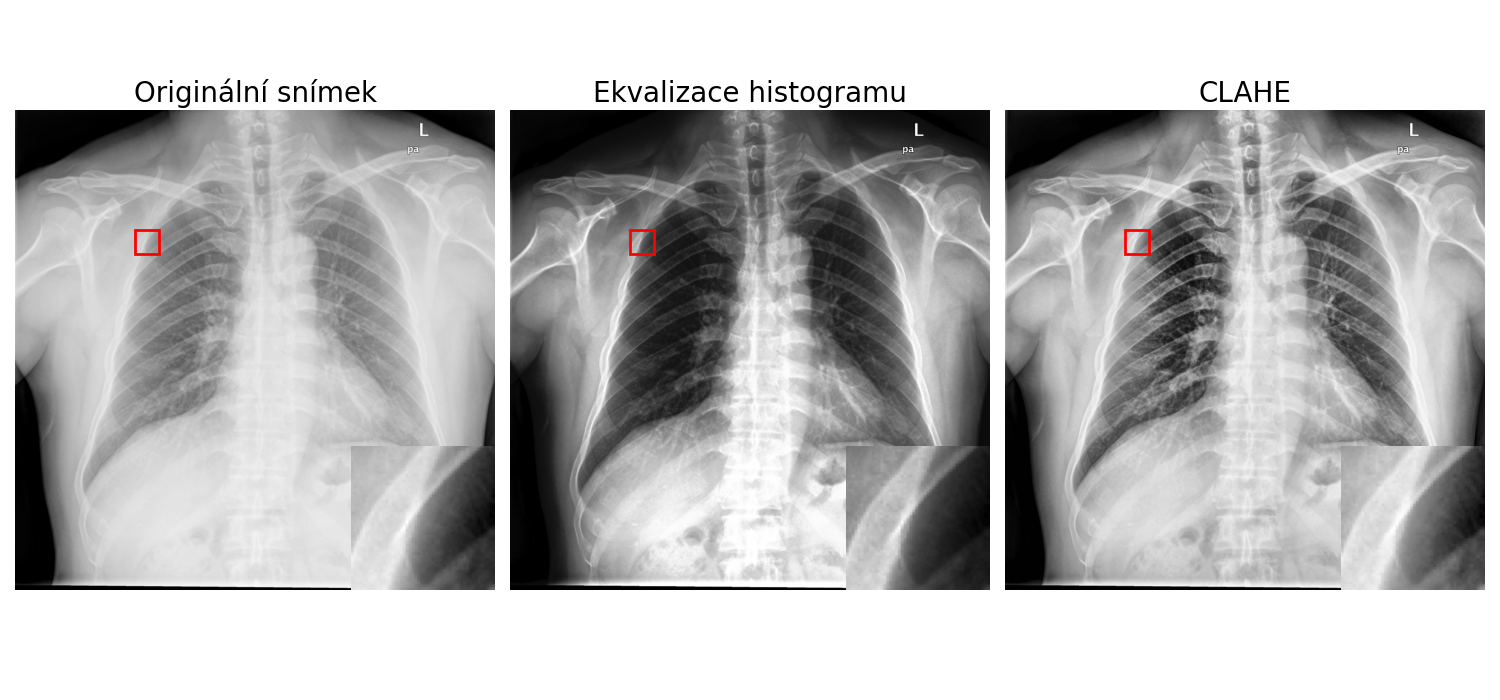
\includegraphics[width=\linewidth]{Prilohy/Obrazky/ImageEnhancement.png}
    \caption{Ukázka metod ekvalizace histogramu na rentgenovém snímku. CLAHE demonstruje lepší zachování detailů a kontrastu v porovnání s tradiční ekvalizací histogramu. (zdrojový snímek převzat z datasetu \cite{LungDataset})}
    \label{fig:histogram_equalization}
\end{figure}

\subsubsection{Unsharp masking}
Unsharp masking je technika určená k zlepšení ostrosti obrazu tím, že zvýrazňuje hrany a detaily, které jsou v původním obrazu méně patrné. Klíčovým krokem této metody je vytvoření tzv. masky ostrých detailů, která vznikne odečtením rozmazané verze obrazu od jeho původní podoby. Rozmazaná verze obrazu se získává například pomocí Gaussova filtru, který je aplikován na původní obraz. Intenzita tohoto rozmazání určuje, jak silně budou hrany a detaily v masce zvýrazněny. Následující rovnice \ref{eq:unsharp_masking} ukazuje získání výsledného, zaostřeného snímku pomocí techniky unsharp masking. Po získání masky ostrých detailů se tato maska přičte zpět k původnímu obrazu. Tento krok zvyšuje kontrast a ostrost obrazu, přičemž zvýrazňuje oblasti s výraznými rozdíly mezi sousedními pixely. \cite{UnsharpMasking}

\begin{equation}
    I_{\text{zaostřený}} = I_{\text{original}} + \lambda \cdot (I_{\text{original}} - I_{\text{rozmazaný}})
    \label{eq:unsharp_masking}
\end{equation}
\begin{conditions}
    I_{\text{original}} & původní obraz \\
    I_{\text{rozmazaný}} & rozmazaná verze původního obrazu \\
    \lambda & faktor určující intenzitu zaostření
\end{conditions}


\begin{algorithm}
    \caption{Unsharp Masking}
    \begin{algorithmic}[1]
        \State \textbf{Vstup:} Původní obraz $I$, standardní odchylka Gaussova filtru $\sigma$, zesílení $\lambda$
        \State \textbf{Výstup:} Vylepšený obraz $I'$
        \State $G \gets \text{Gauss}(I, \sigma)$ \Comment{Vytvoření rozmazané verze obrazu pomocí Gaussova filtru}
        \State $M \gets I - G$ \Comment{Vytvoření masky ostrých detailů odečtením rozmazaného obrazu}
        \State $I' \gets I + \lambda M$ \Comment{Zvýšení ostrosti původního obrazu přičtením masky}
    \end{algorithmic}
\end{algorithm}

V tomto procesu:
\begin{itemize}
    \item $\sigma$ určuje míru rozmazání při použití Gaussova filtru.
    \item $\lambda$ je koeficient zesílení, který kontroluje míru, jakou jsou detaily zvýrazněny při přičítání masky k původnímu obrazu.
\end{itemize}

Při použití unsharp masking metody může vznikat nežádoucí halo efekt. Tento efekt se projevuje jako nežádoucí světelný okraj kolem kontrastních hran, což může vést k umělému a nepřirozenému vzhledu obrazu. Integrace filtru zachovávajícího hrany (edge-preserving filter) do procesu unsharp masking může být klíčová pro minimalizaci zmíněného efektu. \cite{UnsharpMasking}

Unsharp masking metoda je vhodná pro aplikace, kde je žádoucí zlepšit viditelnost detailů a hran. Důležitým aspektem při použití unsharp masking je správný výběr parametrů $\sigma$ a $\lambda$, jelikož tyto hodnoty významně ovlivňují výsledný vzhled obrazu. Příliš vysoké hodnoty mohou vést k nežádoucím artefaktům, jako jsou halo efekty kolem hran, zatímco příliš nízké hodnoty mohou mít za následek nedostatečné zvýraznění detailů.

\subsubsection{Gama korekce}
Gamma korekce je technika používaná k úpravě jasu obrazových dat. Principem této metody je aplikace nelineární transformace na původní pixelové hodnoty obrazu, čímž se upravuje celková jasová křivka podle gamma funkce. Tato korekce umožňuje efektivněji využít dynamický rozsah zobrazovacích zařízení a zlepšit viditelnost detailů v tmavých i světlých oblastech obrazu bez ztráty informací v ostatních částech obrazového spektra. \cite{PreprocessingBook}

Aplikace gamma korekce se obvykle provádí podle vzorce:
\begin{equation}
    I' = I^\gamma
\end{equation}
\begin{conditions}
    I &  původní intenzita pixelu \\
    I' & nová intenzita pixelu po aplikaci gamma korekce \\
    \gamma & gamma faktor, který určuje míru korekce
\end{conditions}

Hodnota gamma faktoru menší než 1 zvýší jas tmavších oblastí obrazu, zatímco hodnota větší než 1 ztmaví světlejší oblasti a zvýší kontrast.
 
\subsection{Redukce šumu}
Redukce šumu ve snímcích je zásadní proces v digitálním zpracování obrazu, který má za cíl odstranit nebo minimalizovat vliv šumu přidaného během akvizice nebo přenosu obrazových dat. Šum může být způsoben různými externími faktory a může výrazně snížit kvalitu a čitelnost snímků, což má negativní dopad na jejich další analýzu a interpretaci.

Šum je obvykle definován jako náhodná variace intenzity obrazových bodů (pixelů), která se projevuje jako viditelné zrnění nebo textura na snímku. Tato náhodná variabilita může být důsledkem základních fyzikálních procesů, jako je povaha fotonu světla nebo tepelná energie v senzorech obrazu. Může vzniknout v okamžiku snímání nebo při přenosu obrazu.

Jednoduchý matematický model, kterým lze vyjádřit přítomnost aditivního šumu v obrazu, můžeme definovat jako:
\begin{equation}
    f(x, y) = I(x, y) + N(x, y)
\end{equation}
\begin{conditions}
    f(x, y) & pozorovaná intenzita pixelu se šumem \\
    I(x, y) & skutečná intenzita pixelu bez šumu \\
    N(x, y) & hodnota šumu přidaná k pixelu
\end{conditions}

Redukce šumu je proto klíčovým krokem ve zpracování obrazu, který pomáhá zlepšit celkovou kvalitu snímků tím, že vyhlazuje obraz a odstraňuje nepřesnosti, avšak s opatrností, aby nedošlo k ztrátě důležitých detailů nebo hran v obrazu. Efektivní algoritmy pro redukci šumu se snaží dosáhnout rovnováhy mezi odstraněním šumu a zachováním nebo dokonce zvýrazněním důležitých vlastností obrazu, jako jsou hrany nebo textury. \cite{ImageDenoisingTechniques,ImageNoiseReductionIran}

\subsubsection{Typy šumu ve snímcích}
Existuje několik typů šumu, které se mohou ve snímcích vyskytovat. Tyto šumy se liší svým původem, charakteristikami a vlivem na kvalitu obrazu. Pro účinnou redukci šumu je klíčové rozpoznat, s jakým typem šumu máme co do činění, aby bylo možné zvolit nejvhodnější metodu pro jeho odstranění. Níže jsou uvedeny některé z nejčastějších typů šumu, které mohou ovlivnit digitální snímky.

\begin{itemize}
    \item \textbf{Gaussovský šum} je pravděpodobně nejrozšířenějším typem šumu v digitálních obrazových systémech, způsobený především elektronickými fluktuacemi v senzoru a obvodech kamery. Je charakterizován normálním rozdělením intenzit pixelů kolem skutečné hodnoty s určitou střední hodnotou a standardní odchylkou. \[P(n) = \frac{1}{\sqrt{2\pi\sigma^2}} e^{-\frac{(n-\mu)^2}{2\sigma^2}}\] Gaussovský šum je obvykle považován za aditivní šum, což znamená, že jeho hodnota je nezávisle přidána k intenzitě každého pixelu. \cite{ImageDenoisingTechniques}
    \item \textbf{Impulzní šum (Šum soli a pepře)} se projevuje jako náhodné černé nebo bílé (nebo obojí) pixely rozptýlené po celém obrazu. Tento typ šumu může vzniknout kvůli chybám v senzoru nebo při přenosu dat. Na rozdíl od Gaussovského šumu je impulzní šum typicky nelineární a jeho redukce vyžaduje specifické nelineární filtrační techniky. \cite{ImageDenoisingTechniques}
    \item \textbf{Poissonův šum} je typ šumu, který je často přítomen v obrazových datech získaných z nízkých intenzit světla, jako jsou rentgenové snímky nebo mikroskopické snímky. Poissonův šum je důsledkem náhodného procesu počtu fotonů, které dopadají na senzor, a je charakterizován jako náhodný proces s diskrétním rozdělením pravděpodobnosti. Redukce Poissonova šumu vyžaduje specifické metody, které jsou schopny zacházet s diskrétními daty a zároveň zachovat důležité detaily v obraze. \cite{ImageDenoisingTechniques} Poissonův šum může být modelován jako: \[ P(n) \sim \frac{e^{-\lambda} \lambda^n}{n!}\] 
    \item \textbf{Speckle šum} se řadí do skupiny multiplikativních šumů, které jsou často přítomny v ultrazvukovém a radarovém zobrazování. Tento šum je důsledkem koherence vlnění použitého pro snímání a interferencí mezi rozptýlenými vlnami. Speckle šum může být modelován pomocí Rayleighova nebo Gamma rozdělení v závislosti na povaze obrazových dat. \cite{ImageDenoisingTechniques}
\end{itemize}

\subsubsection{Typy filtrů pro redukci šumu}
Pro efektivní redukci šumu ve snímcích jsou k dispozici různé typy filtrů, které se liší svým principem a účinností v závislosti na konkrétním typu šumu. Filtrování šumu se dělí na:

\begin{itemize}
    \item \textbf{Lineární filtrování}, také známo jako konvoluční filtrování, aplikuje lineární operátor na skupinu sousedících pixelů v obrazu s cílem vyhladit nebo zvýraznit určité vlastnosti obrazu. Hlavní principem lineárních filtrů je konvoluce obrazu s jádrem filtru či maskou, což je malá matice daného rozměru, která určuje váhy pro každý pixel v okolí. Tyto váhy určují, jakým způsobem okolní pixely ovlivňují hodnotu pixelu výstupního obrazu. Hlavní výhodou lineárních filtrů je jejich jednoduchost a efektivita, což je dělá vhodnými pro rychlé a efektivní zpracování obrazu. Nicméně, lineární filtry mohou způsobovat neostrost hran a detailů ve snímcích. \cite{ImageDenoisingTechniques, XRayImageProcessing}
    
    \begin{equation}
        I_{filtered}(x, y) = \sum_{i=-a}^{a} \sum_{j=-b}^{b} K(i, j) \cdot I(x-i, y-j)
    \end{equation}
    \begin{conditions}
        I_{filtered}(x, y) & intenzita pixelu na pozici (x, y) ve filtrovaném snímku \\
        K(i, j) & koeficienty konvoluční masky (kernelu) \\
        I(x-i, y-j) & intenzita pixelu v původním snímku v okolí pixelu (x, y) 
    \end{conditions}
    \item \textbf{Nelineární filtrování} je alternativní přístup k redukci šumu, který se zaměřuje na zachování hran a detailů v obraze. Nelineární filtry jsou schopny zacházet s nelineárními vztahy mezi pixely a jsou schopny lépe zachovat důležité strukturální vlastnosti obrazu. Nelineární filtry jsou proto obzvláště účinné při redukci impulzního či speckle šumu. \cite{ImageDenoisingTechniques, XRayImageProcessing}
\end{itemize}

Níže jsou uvedeny některé z nejčastěji používaných filtrů pro redukci šumu ve snímcích a na obrázku \ref{fig:noise_reduction_filters} je předvedeno jejich použítí.

\subsubsection{Gaussovský filtr}
Gaussovský filtr reprezentuje jeden z nejčastěji používaných lineárních filtrů pro redukci šumu ve snímcích. Tento filtr je založen na aplikaci Gaussova jádra na obraz. Jádro, někdy nazýváno kernel, je symetrická matice s hodnotami vygenerovanými podle dvourozměrné Gaussovské funkce, která se používá pro konvoluci s obrazem za účelem dosažení efektu vyhlazení, kde středové pixely mají největší váhu a váha se snižuje s rostoucí vzdáleností od středu, což vede k účinnému potlačení vysokofrekvenčního šumu. Gaussovský filtr je definován vzorcem:

\begin{equation}
    G(x, y) = \frac{1}{2\pi\sigma^2} e^{-\frac{x^2 + y^2}{2\sigma^2}}
\end{equation}
\begin{conditions}
    G(x, y) & hodnota Gaussova jádra na pozici (x, y) \\
    \sigma & standardní odchylka Gaussova jádra
\end{conditions}

Gaussovský filtr je schopen efektivně redukovat Gaussovský šum a jednou z hlavních výhod je jeho přirozená odezva na vysokofrekvenční oblasti, které potlačuje bez vytváření kroužkových artefaktů, které jsou běžné u low-pass filtrů.

Přestože je Gaussovský filtr velmi účinný při redukci šumu, volba směrodatné odchylky $\sigma$ je kritická. Příliš vysoká hodnota může vymazat důležité detaily spolu se šumem, zatímco příliš nízká hodnota nemusí šum dostatečně snížit. Navíc, izotropní povaha Gaussovského filtru znamená, že filtr rozmazává ve všech směrech stejnou měrou, což nemusí být žádoucí zejména tam, kde je potřeba zachování hran. \cite{XRayImageProcessing}

\begin{algorithm}
    \caption{Gaussovský filtr}
    \begin{algorithmic}[1]
        \State \textbf{Vstup:} Původní obraz $I$, standardní odchylka $\sigma$
        \State \textbf{Výstup:} Vyhlazený obraz $I_{smoothed}$
        \State Vytvořte Gaussovo jádro $G$ s rozměry $n \times n$ a $\sigma$
        \State \textbf{Inicializuj} $I_{smoothed}$ jako prázdný obraz
        \For{každý pixel $p$ v $I$}
            \State Aplikujte Gaussovo jádro na okolí pixelu $p$
            \State Nastavte hodnotu pixelu $p$ v $I_{smoothed}$ na vážený průměr hodnot v okolí
        \EndFor
        \State \textbf{return} $I_{smoothed}$
    \end{algorithmic}
\end{algorithm}

\subsubsection{Bilaterální filtr}
Bilaterální filtrování je nelineární technika pro vyhlazování obrazu, která zachovává hrany a redukuje šum (metoda se specializuje na redukci Gaussovského šumu). Na rozdíl od tradičních lineárních filtrů, které aplikují uniformní konvoluci napříč obrazem, bilaterální filtr kombinuje dva hlavní koncepty: prostorovou blízkost a podobnost intenzity. 

Podobně jako Gaussův filtr, bilaterální filtr používá Gaussovu funkci k vážení pixelů, založené na prostorové vzdálenosti pixelů od centrálního pixelu. Tím pádem, čím jsou pixely blíže k centrálnímu pixelu, tím větší váhu mají. Unikátní pro bilaterální filtr je fakt, že váhy jsou také přizpůsobeny na základě rozdílu intenzit mezi sousedními pixely a centrálním pixelem. Pixely s podobnou intenzitou jako centrální pixel získávají vyšší váhu, což umožňuje zachování ostrých hran a detailů. Pro každý pixel ve zpracovávaném obrazu filtr vyhodnotí jeho sousedy a aplikuje váhy založené na dvou zmíněných kritériích. \cite{BilateralFilter}

Matematický vzorec pro bilaterální filtr aplikovaný na obraz lze vyjádřit jako:
\begin{equation}
    BF[I](p) = \frac{1}{W_p} \sum_{q \in S} G_{\sigma_s}(||p-q||) \cdot G_{\sigma_r}(|I_p - I_q|) \cdot I_q
\end{equation}
\begin{conditions}
    BF[I](p) & hodnota pixelu po aplikaci bilaterálního filtru \\
    W_p & je normalizační faktor zajišťující, že součet vah je roven jedné \\
    G_{\sigma_s} & prostorová Gaussova funkce, která snižuje vliv vzdálených pixelů na základě prostorové vzdálenosti $||p-q||$ se standardní odchylkou $\sigma_s$ \\
    G_{\sigma_r} & rozsahová Gaussova funkce, která redukuje vliv pixelů $q$ na základě rozdílu intenzit $|I_p-I_q|$ se standardní odchylkou $\sigma_r$ \\
    S & sousední pixely zpracovávaného pixelu $p$ \\
    I_p & hodnota pixelu $p$ \\
    I_q & hodnota pixelu $q$ \\
\end{conditions}

\begin{equation}
    W_p = \sum_{q \in S} G_{\sigma_s}(||p-q||) \cdot G_{\sigma_r}(|I_p - I_q|)
\end{equation}

Na rozdíl od Gaussova filtru, který aplikuje vyhlazování uniformně a může vést k rozmazání ostrých hran, bilaterální filtr nabízí sofistikovanější přístup k redukci šumu. Jeho schopnost zachovat ostré hrany při současném snížení šumu v homogenních oblastech obrazu činí bilaterální filtr vysoce ceněným nástrojem v pokročilém zpracování obrazu. Avšak, s touto schopností přichází zvýšená výpočetní náročnost a potřeba pečlivého nastavení parametrů $\sigma_s$ a $\sigma_r$, což jsou aspekty, které je třeba zvážit pro dosažení optimálních výsledků. \cite{BilateralFilter}

\subsubsection{Wienerův filtr}
Wienerův filtr je adaptivní lineární filtr, který je často používán pro redukci aditivního šumu ve snímcích s cílem zachovat důležité detaily a strukturální vlastnosti obrazu. Wienerův filtr funguje na principu minimalizace střední kvadratické chyby (anglicky minimum mean squared error - MMSE)\footnote{MSE je metrika, která měří rozdíl mezi odhadovanými a skutečnými hodnotami. V případě Wienerova filtru se minimalizuje rozdíl mezi původním obrazem a obrazem se šumem.} mezi původním obrazem a obrazem se šumem. Matematicky je Wienerův filtr navržen tak, aby našel spektrální rovnováhu mezi inverzním filtrováním signálu a vyhlazováním šumu, s ohledem na výkonová spektra signálu a šumu. Odezva filtru je vypočítána pomocí výkonových spekter, což vede k optimálnímu vyvážení mezi inverzním filtrováním pro obnovu obrazu a potlačením šumu.

\begin{equation}
    G(u,v) = \frac{1}{H(u,v)} \left[ \frac{\left| H(u,v) \right|^2}{\left| H(u,v) \right|^2 + \frac{S_{\eta}}{S_f}} \right]
\end{equation}
\begin{conditions}
    G(u,v) & odhad originálního obrazu \\
    H(u,v) & degradační funkce \\
    S_{\eta} & výkonové spektrum šumu \\
    S_f & výkonové spektrum originálního obrazu
\end{conditions}

Tento vztah představuje schopnost Wienerova filtru vyvažovat mezi inverzním filtrováním a vyhlazováním šumu s ohledem na degradační funkci a poměr signálu a šumu $\frac{S_{\eta}}{S_f}$\footnote{Poměr signálu a šumu (SNR) udává poměr mezi obrazem a úrovní šumu v daném obraze. Vysoká hodnota SNR značí, že signál je silnější než šum, což znamená, že obraz má vysokou kvalitu s minimálním množstvím šumu. Naopak nízká hodnota SNR indikuje, že šum je dominantní a signál je obtížně rozeznatelný.}. Filtr je více nakloněn k inverznímu filtrování, kde je magnituda degradační funkce velká vzhledem k šumu (vysoké SNR), a více k vyhlazování v opačném případě. \cite{WienerFilters}

\subsubsection{Mediánový filtr}
Mediánový filtr je robustní nelineární filtrační technika, který se používá k redukci impulzního šumu (šumu soli a pepře). Mediánový filtr funguje tak, že posouvá okno po každém pixelu obrazu, shromažďuje hodnoty pixelů z okolí daného pixelu a nahrazuje středový pixel mediánem těchto hodnot. Okno, které se obvykle používá, je čtvercové (např. 3x3, 5x5) v závislosti na stupni šumu a požadované úrovni zachování detailů. Na rozdíl od průměrových filtrů, které také snižují šum, ale mají tendenci rozmazávat hrany, mediánový filtr hrany zachovává. Dále také mediánový filtr nezávisí na předpokladu, že šum je specifického typu nebo variance.

\begin{algorithm}
    \caption{Mediánový filtr}
    \begin{algorithmic}[1]
        \State \textbf{Vstup:} Původní obraz $I$, velikost okna $k$
        \State \textbf{Výstup:} Obraz po redukci šumu $I_{filtered}$
        \State \textbf{Inicializuj} $I_{filtered}$ jako prázdný obraz
        \For{každý pixel $p$ v $I$}
            \State \text{okolí} $\gets$ \text{extrahuj\_okolí}($I$, $p$, $k$)
            \State \text{medián} $\gets$ \text{vypočti\_medián}(okolí)
            \State \text{Nastavte hodnotu pixelu} $p$ v $I_{filtered}$ na \text{medián}
        \EndFor
        \State \textbf{return} $I_{filtered}$
    \end{algorithmic}
\end{algorithm}

Přestože je mediánový filtr účinný, má svá omezení, zejména při vysokých úrovních šumu nebo když mají obrazy jemné strukturální detaily. Za těchto podmínek může filtr odstranit užitečné informace spolu se šumem. Navíc jeho výkon se může zhoršit, pokud není velikost okna správně zvolena, protože příliš velké okno může odstranit příliš mnoho detailů, zatímco příliš malé okno nemusí efektivně odstranit dostatek šumu.

\subsubsection{Filtr ne-lokálních průměrů}
Filtr ne-lokálních průměrů, anglicky Non-Local Means (NLM), představuje pokročilou techniku pro odstranění šumu z obrazu (převážně Gaussovského šumu), která se vyznačuje výrazným zachováním detailů a hran. Na rozdíl od tradičních metod, které pracují s lokálními okolími pixelů, NLM vyhledává podobné fragmenty (patche) po celém obrazu a využívá jejich informace pro inteligentní vyhlazení cílového pixelu nebo oblasti, čímž se minimalizuje ztráta důležitých vizuálních prvků. NLM můžeme rozdělit na dvě varianty: pixelwise a patchwise NLM.

První varianta, pixelwise NLM, se zaměřuje na každý pixel individuálně. Pro každý pixel $p$ ve vstupním obraze 
$I$ se vypočítává jeho nová hodnota jako vážený průměr hodnot všech pixelů v obraze. Váhy závisí na podobnosti malých okolí (patchů) okolo každého pixelu a jsou určeny Euklidovskou vzdáleností mezi hodnotami pixelů v těchto okolích. Matematicky lze pixelwise NLM vyjádřit pomocí vztahu:

\begin{equation}
    I_{new}(p) = \frac{\sum_{q \in I} w(p,q) \cdot I(q)}{\sum_{q \in I} w(p,q)}
\end{equation}
\begin{conditions}
    w(p,q) & představuje váhu založenou na podobnosti mezi okolím pixelů $p$ a $q$ \\
    I(q) & hodnota pixelu $q$ ve vstupním obraze
\end{conditions}

Druhá varianta, patchwise NLM, rozšiřuje přístup pixelwise metody tím, že jako základní jednotku pro výpočet váženého průměru bere celé patche namísto jednotlivých pixelů. Tím se zvyšuje robustnost metody vůči šumu, jelikož se lépe využívá strukturální informace z obrazu. Vztah pro patchwise NLM může být zapsán obdobně, avšak s důrazem na porovnávání celých patchů.

Rozdíl mezi pixelwise a patchwise variantami spočívá v měřítku, na kterém se hodnotí podobnost mezi částmi obrazu. Zatímco pixelwise varianta se soustředí na detailní porovnání na úrovni pixelů, patchwise přístup poskytuje robustnější odhad tím, že zapojuje větší kontext okolí zkoumaného bodu.

Algoritmus NLM, ať už v pixelwise či patchwise variantě, nabízí vynikající schopnost odstraňování šumu při zachování ostrých hran a detailů. Jeho hlavní nevýhodou však zůstává vysoká výpočetní náročnost, zejména v důsledku nutnosti porovnávat velké množství oblastí napříč celým obrazem. To činí aplikaci NLM, především v reálném čase, výzvou. Optimalizace a využití paralelního zpracování však mohou tuto nevýhodu zmírnit. \cite{NonLocalMeans}

\subsubsection{Lokálně adaptivní mediánový filtr}
Lokálně adaptivní mediánový filtr je inovativní metodou redukce šumu, specificky navrženou pro typ šumu speckle. Tento typ šumu je výsledkem interferencí mezi koherentními vlnami odraženými od cíle, což vede k zrnitému vzoru v pořízeném obraze. Tento filtr využívá lokální statistiky pro detekci speckle šumu a jeho nahrazení mediánovou hodnotou z lokálního okolí.

Nejdříve je nutné zjistit celkový součet intenzit pixelů v určitém oblastním okně, které obklopuje centrální pixel. Tento součet je základem pro další výpočty statistik, jako je lokální průměr.
\begin{equation}
    S(i, j) = \sum_{n=j-k}^{j+k}\sum_{m=i-k}^{i+k} d(m, n)
\end{equation}
\begin{conditions}
    k & poloměr posuvného okna okolo středového pixelu \\
    d(m, n) & hodnota pixelu na pozici $(m, n)$
\end{conditions}

Dále se určí průměrná hodnota a lokální standardní odchylka hodnot pixelů v posuvném okně. Lokální průměr pomáhá rozlišit oblasti s vysokým a nízkým šumem tím, že poskytuje základní hodnotu pro porovnání s ostatními pixely. Standardní odchylka je míra variability nebo rozptylu hodnot pixelů kolem lokálního průměru, která pomáhá identifikovat pixely s výrazně odlišnými intenzitami (tj. šum).
\begin{equation}
    \mu(i, j) = \frac{S(i, j)}{N(i, j)}
\end{equation}
\begin{conditions}
    S(i, j) & součet všech hodnot pixelů v posuvném okně \\
    N(i, j) = (2k + 1)^2 & počet pixelů v posuvném okně
\end{conditions}

\begin{equation}
    \sigma(i, j) = \sqrt{\frac{\sum_{m=i-k}^{i+k} \sum_{n=j-k}^{j+k} (d(m, n) - \mu(i, j))^2}{N(i, j)}}
\end{equation}
\begin{conditions}
    \mu(i, j) & lokální průměr hodnot pixelů v posuvném okně
\end{conditions}

Na základě definované dolní a horní hranice pro rozpoznání validních pixelů v rámci posuvného okna se rozhodne, které pixely jsou považovány za validní, a které představují potenciální šum.
\begin{equation}
    \begin{split}
        LB(i, j) &= \mu(i, j) - M \cdot \sigma(i, j) \\
        UB(i, j) &= \mu(i, j) + M \cdot \sigma(i, j)
    \end{split}
\end{equation}
\begin{conditions}
    \mu(i, j) & lokální průměr hodnot pixelů v posuvném okně \\
    \sigma(i, j) & lokální standardní odchylka hodnot pixelů v posuvném okně \\
    M & uživatelem definovaný násobitel pro určení prahu šumu
\end{conditions}

\begin{equation}
    l(m, n) = 
    \begin{cases} 
        0 & \text{pokud } d(m, n) < LB(i, j) \text{ nebo } d(m, n) > UB(i, j) \\
        1 & \text{pokud } LB(i, j) \leq d(m, n) \leq UB(i, j)
    \end{cases}
\end{equation}
\begin{conditions}
    LB(i, j), \ UB(i, j) & dolní a horní hranice pro validní hodnoty pixelů
\end{conditions}

Finální rovnice nahrazuje hodnotu centrálního pixelu, identifikovaného jako šum, mediánovou hodnotou z validních pixelů v okně. Tento proces zajišťuje, že hodnota pixelu reprezentuje jeho skutečné okolí a zlepšuje tak celkovou kvalitu obrazu redukcí šumu.
\begin{equation}
    r(i, j) = \text{median } d(m, n) \text{ | } l(m, n) = 1, i-k \le m, n \le i+k
\end{equation}
\begin{conditions}
    l(m, n) & maska určující, zda je pixel na pozici $(m, n)$ považován za validní nebo za šum
\end{conditions}

Lokálně adaptivní mediánový filtr se ukazuje jako výrazně efektivní při odstraňování speckle šumu, což je běžný problém v rentgenových a jiných druzích medicínských snímků. Využití lokálních statistik umožňuje filtru selektivně cílit na šumové pixely, zatímco zachovává ostré hrany a důležité detaily, což je klíčové pro zachování diagnostické hodnoty obrazu.

Nicméně, stejně jako většina pokročilých metod zpracování obrazu, i tento filtr má své nevýhody. Především je to jeho výpočetní náročnost, která může být limitující pro aplikace v reálném čase nebo při zpracování velkých datasetů. Navíc, efektivní využití filtru vyžaduje pečlivý výběr parametrů, což může vyžadovat pokročilé znalosti a experimentální ladění pro dosažení optimálních výsledků. \cite{LocalAdaptiveMedianFilter}

\begin{figure}[H]
    \centering
    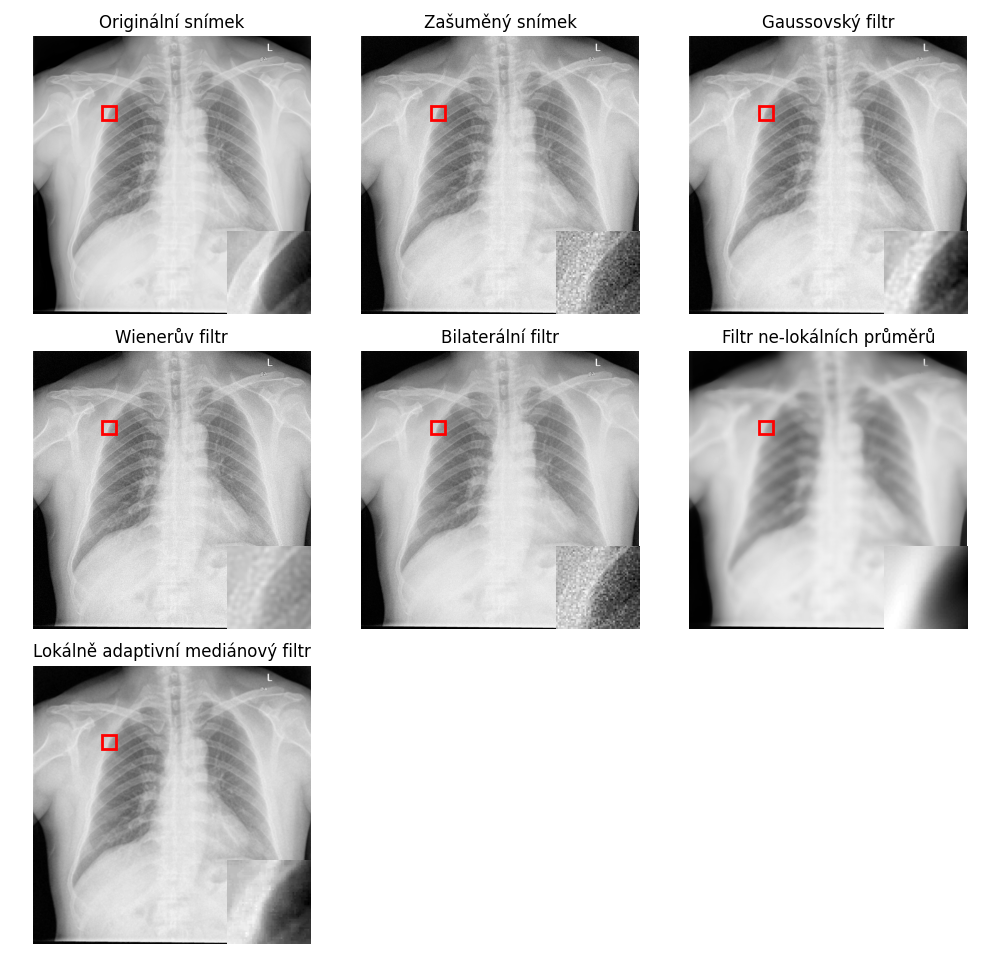
\includegraphics[width=\linewidth]{Prilohy/Obrazky/NoiseReduction.png}
    \caption{Snímky demonstrují účinky popsaných filtrů na kvalitu obrazu v porovnání s originálním snímkem a snímkem po umělém přidání šumu, aby se simulovalo běžné zkreslení vznikající během akvizice obrazu. (zdrojový snímek převzat z datasetu \cite{LungDataset})}
    \label{fig:noise_reduction_filters}
\end{figure}

\subsection{Výzvy a úskalí standardních metod}
Standardní metody pro odstranění šumu mají několik omezení, která mohou ovlivnit jejich účinnost v reálných aplikacích. Tato omezení jsou důležitá pro pochopení, proč samotné použití těchto metod nemusí být vždy dostatečné a proč je třeba hledat pokročilejší přístupy.

Většina standardních metod je navržena tak, aby se zaměřovala na specifické typy šumu. Například mediánový filtr je efektivní pro odstranění impulzního šumu, ale nemusí být účinný proti jiným typům. Toto zaměření na specifické typy šumu znamená, že pokud není typ šumu v obraze znám, může být obtížné vybrat správnou metodu pro jeho odstranění. V reálných aplikacích často není možné předem určit, jaký typ šumu bude v obraze přítomen, což výrazně omezuje účinnost těchto metod.

Dalším problémem je přítomnost více typů šumu současně v jednom obraze. Například, lékařské snímky mohou obsahovat kombinaci šumu typu speckle, Poissonova šumu a dalších artefaktů \cite{MostCommonNoises}. Standardní metody, které jsou navrženy pro odstranění jednoho typu šumu, nemusí být schopny efektivně zvládnout takovou kombinaci. Použití jedné metody může zlepšit jednu část obrazu, ale zároveň zhoršit jinou. Tento problém kombinace šumů vede k potřebě metod, které jsou schopny efektivně řešit více typů šumu současně, nebo metod, které kombinují výstupy různých filtrů pro dosažení lepších výsledků.

\section{Neuronové sítě pro předzpracování obrazu}
Předchozí sekce byla věnována klasickým metodám předzpracování obrazu, kde byl brán důraz na techniky pro vylepšení obrazu a odstranění či redukci různých typů šumu ze snímků. Tato sekce se bude zabývat pokročilým oborem pro předzpracování obrazu, kterým jsou neuronové sítě.

Neuronové sítě představují významný skok v možnostech zpracování obrazu, především díky jejich schopnosti učit se a generalizovat na základě velkých datových sad. Na rozdíl od klasických metod, které aplikují pevně stanovená pravidla, se neuronové sítě dokáží přizpůsobit na základě konkrétních charakteristik a variací v datech, na kterých jsou trénovány. Tato adaptabilita je klíčová pro zpracování obrazů v dynamických a různorodých podmínkách, což zahrnuje vše od standardního zlepšování obrazu po složité úlohy jako je rozpoznávání objektů nebo segmentace obrazu.

Neuronové sítě, a zvláště konvoluční neuronové sítě (CNN), jsou vysoce efektivní v automatickém učení a rozpoznávání vzorců z obrazových dat. Tyto sítě simulují způsob, jakým lidský mozek zpracovává vizuální informace, což umožňuje extrakci a učení vysokého řádu charakteristik, které jsou následně využity pro klasifikaci nebo predikci. Díky této schopnosti se neuronové sítě stávají základem mnoha pokročilých systémů pro automatizované zpracování obrazu.

Využití neuronových sítí však také přináší výzvy, včetně potřeby velkého množství anotovaných trénovacích dat a výpočetně náročných modelů, které mohou vyžadovat specializovanou hardwarovou podporu pro efektivní trénink a nasazení. 

Následující sekce bude zaměřena na nejčastěji využívané architekty neuronových sítí pro předzpracování obrazu, s důrazem na konvoluční neuronové sítě (CNN). \cite{CNNConcepts}

\subsection{Úvod do konvolučních neuronových sítí}
Neuronové sítě jsou základním stavebním prvkem moderního strojového učení a mají zásadní význam pro rozvoj oblastí jako je zpracování přirozeného jazyka či obrazu, rozpoznávání objektů v obraze, při analýze signálu, v robotice a mnoha jiných důležitých oborech. Tyto systémy jsou inspirovány strukturou a funkcí lidského mozku a jsou navrženy tak, aby modelovaly složité vzory a vztahy v datech. Strukturálně jsou neuronové sítě složeny z vrstev neuronů, což jsou jednotky zpracovávající informace, které jsou propojeny spojeními, ohodnocenými vahami. Tento vztah je ilustrován na obrázku \ref{fig:nn_components}.

\begin{figure}[H]
    \centering
    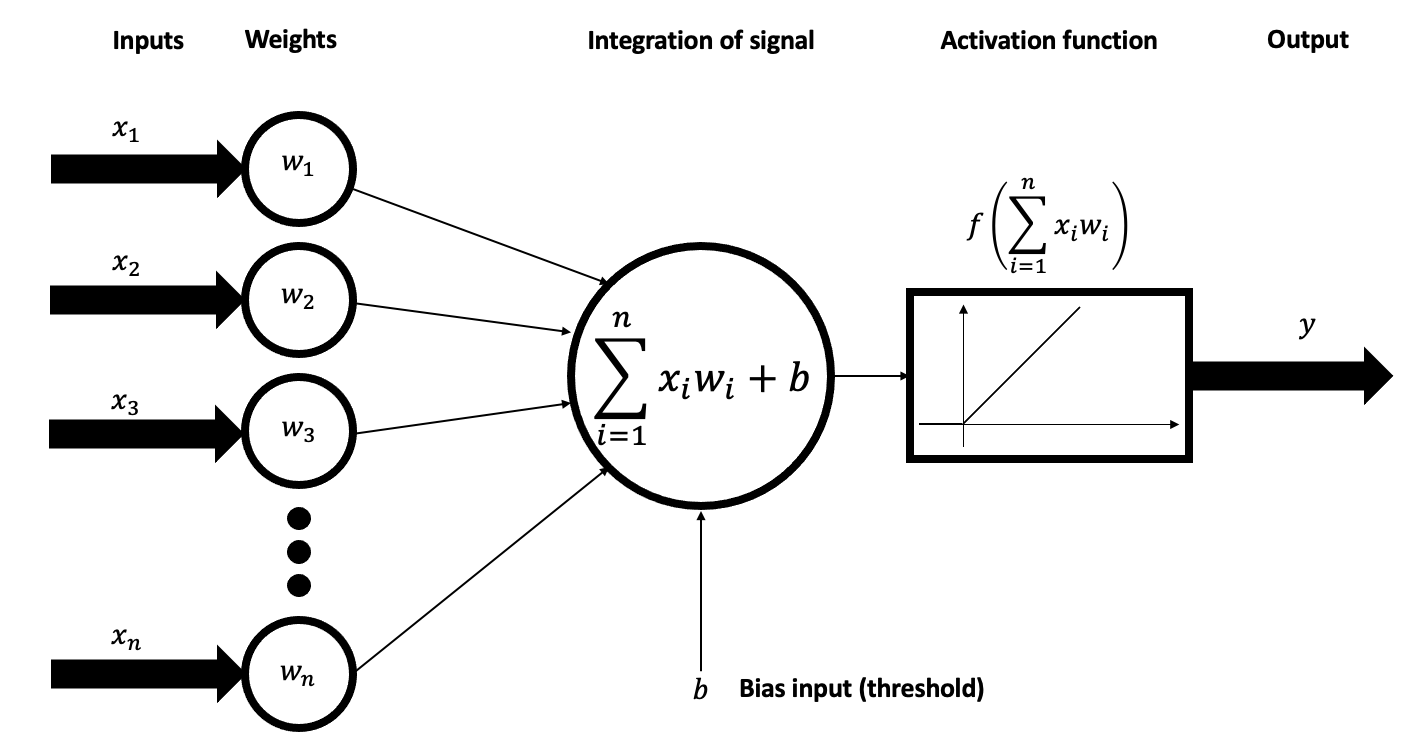
\includegraphics[width=\linewidth]{Prilohy/Obrazky/NNComponents.png}
    \caption{Ilustrace neuronové jednotky, ukazující základní komponenty jako vstup, váhy, bias, aktivační funkci a výstup. (převzato z \cite{NNComponentsIMG} pod licencí CC BY-SA 4.0)}
    \label{fig:nn_components}
\end{figure}

\subsubsection{Hlavní komponenty neuronových sítí}
Základem neuronové sítě je její architektura, která je definována několika klíčovými komponentami. Tyto komponenty jsou základem pro učení a zpracování dat v síti. V následujícím seznamu jsou jednotlivé komponenty podrobněji popsány:

\begin{itemize}
    \item \textbf{Neuron} je elementární jednotka v neuronové síti, která simuluje chování neuronu v biologických systémech. Přijímá vstup $x = (x_1, x_2, x_3, ..., x_n)$, který je zpracován a následně vrácen na výstupu. Tento výstup je vstupem do dalšího neuronu nebo je součástí koncového výstupu ze sítě.
        \begin{equation}
            z = W \cdot x + b
        \end{equation}
        \begin{conditions}
            W & reprezentuje váhy, jež jsou parametry určující sílu signálu mezi neurony. \\
            b & bias, což je parametr posunutí, který upravuje výstup neuronu před aplikací aktivační funkce.
        \end{conditions}
    \item \textbf{Vrstvy (Layers)} se skládají z neuronů a jsou základem architektury neuronové sítě. Každá vrstva plní specifickou funkci v procesu učení. Vrstvy mohou být kategorizovány do tří typů:
        \begin{itemize}
            \item \textbf{Vstupní vrstva (Input layer)} přijímá surová data a připravuje je pro další zpracování v síti. Každý neuron této vrstvy přímo reprezentuje jednu vlastnost vstupního datového vektoru.
            \item \textbf{Skyté vrstvy (Hidden layers)} jsou mezi vstupní a výstupní vrstvou a jejich úkolem je zpracování signálů přijatých od vstupní vrstvy. Komplexnost a hloubka těchto vrstev jsou klíčové pro schopnost sítě učit se složité vzory.
            \item \textbf{Výstupní vrstva (Output layer) } je poslední vrstva, která generuje predikce určené neuronovou sítí. Například v klasifikačních úlohách může tato vrstva používat softmax funkci\footnote{Softmax funkce se často používá jako aktivační funkce v poslední vrstvě neuronové sítě při klasifikačních úlohách. Tato funkce převádí výstupní hodnoty neuronů na pravděpodobnostní rozdělení mezi různými třídami. Matematický vzorec pro softmax funkci je definován následovně: $\text{softmax}(z_i) = \frac{e^{z_i}}{\sum_{j=1}^{N} e^{z_j}}$}.
        \end{itemize}
    \item \textbf{Aktivační funkce (Activation function)} je důležitou složkou neuronových sítí, která umožňuje modelování nelineárních vztahů. Funkce, jako je logistická funkce (sigmoid), hyperbolický tangens (tanh) a ReLU (Rectified Linear Unit), jsou běžně používány k výpočtu výstupu z neuronů na základě vstupu a vah. Například, ReLU, která je definována jako $ReLU(x) = max(0, x)$, je populární pro svou schopnost rychle konvergovat během tréninku a minimalizovat problém mizejících gradientů\footnote{Mizející gradienty jsou problém, kdy gradient ztrátové funkce klesá exponenciálně rychle s každou vrstvou v síti, což způsobuje, že váhy v raných vrstvách se téměř neaktualizují. Tento jev výrazně zpomaluje trénink a může způsobit, že síť nedokáže efektivně učit složité vzory.}.
    \item \textbf{Ztrátová funkce (Loss function)}, někdy nazývaná penalizační funkce, poskytuje kvantitativní hodnocení toho, jak daleko jsou predikce neuronové sítě od skutečných hodnot. Během tréninku neuronové sítě je hlavním cílem minimalizace této funkce. Mezi běžné ztrátové funkce se řadí střední kvadratická chyba (MSE) pro regresní úkoly a cross-entropy pro klasifikační úkoly. 
    \item \textbf{Optimalizační algoritmus (Optimizer)} je základem učení neuronových sítí, protože určují, jak se síť učí z dat tím, že iterativně upravují váhy a biasy k minimalizaci ztrátové funkce. Stochastic Gradient Descent (SGD) provádí tuto úpravu tak, že v každém kroku tréninku náhodně vybere vzorek dat a spočítá gradient ztrátové funkce pouze na základě tohoto vzorku:
    Adam a RMSprop jsou pokročilejší varianty, které se snaží zlepšit konvergenci SGD tím, že upravují rychlost učení pro každý parametr individuálně, což může vést k rychlejšímu a stabilnějšímu učení, zejména v komplexních sítích.
\end{itemize}

Základní komponenty neuronových sítí hrají zásadní roli ve funkcionalitě vytvořených modelů. Neurony a vrstvy formují strukturu sítě, zatímco aktivační funkce umožňují modelování nelineárních vztahů, což je nezbytné pro zpracování složitých vzorů a funkcí. Ztrátové funkce poskytují metriku pro hodnocení úspěšnosti sítě v předpovídání a jsou klíčové pro navigaci procesu učení. Optimalizační algoritmy řídí tento učící se proces tím, že iterativně upravují interní parametry sítě, aby se minimalizovala celková ztráta a zvýšila přesnost modelu. Každá z těchto komponent společně zajišťuje, že neuronové sítě se mohou učit efektivně, adaptovat se a poskytovat přesné predikce při řešení zadaných úloh. \cite{CNNConcepts, CNNConcepts2}

\subsubsection{Základy konvolučního zpracování v CNN}
Jak již bylo zmíněno výše, konvoluční neuronové sítě (CNN) jsou specializovaným druhem neuronových sítí, které se používají především pro zpracování strukturovaných dat, jako jsou například obrazová data. CNN jsou známé svou schopností zachytit prostorové a časové závislosti v obraze pomocí aplikace příslušných filtrů. Úloha konvolučních operací je jádrem toho, co činí CNN tak efektivními pro úlohy, jako je rozpoznávání obrazu, klasifikace obrazu a detekce objektů.

Operace konvoluce zahrnuje posunutí jádra (kernelu) přes vstupní data (obvykle obraz) a výpočet skalárního součinu jádra s překrývajícími se části obrazu. Výsledek tvoří jednu položku ve výstupní mapě příznaků. Tento proces se opakuje posouváním jádra po všech pozicích vstupní matice. Mezi klíčové aspekty konvoluce patří:

\begin{itemize}
    \item \textbf{Jádro konvoluce} Malé matice používané k detekci specifických prvků, jako jsou hrany nebo textury ve vstupním obraze. Každý filtr je navržen tak, aby zachytil určitý aspekt vstupních dat.
    \item \textbf{Krok jádra} Počet pixelů, o které posouváme filtr po vstupním obraze. To ovlivňuje velikost výstupní mapy prvků.
    \item \textbf{Padding} Existuje několik možností, jak umožnit jádru brát v potaz i hraniční prvky. Jednou z možnosti je přidání vrstev nul kolem vstupního obrazu. Další možností je použití zrcadlení (mirror padding), kde se okrajové prvky zrcadlově opakují, což pomáhá jádru zahrnout informace z okrajů obrazu bez ztráty dat.
    \item \textbf{Mapa příznaků} Výstup operace konvoluce se nazývá mapa příznaků. Představuje odezvu filtru v každé prostorové poloze. Použitím různých filtrů může síť CNN zachytit širokou škálu aspektů vstupního obrazu.
\end{itemize}

Dalším důležitým konceptem v CNN je tvz. pooling, které se obvykle používá po operaci konvoluce. Nejběžnější formou sdružování je max pooling, kde výstupem sdružovacího jádra je maximální hodnota z části mapy, kterou pokrývá. Tato operace snižuje dimenzionalitu mapy příznaků a umožňuje síti být odolnou vůči malým změnám vstupního obrazu.

V hlubokých konvolučních neuronových sítích se vrství několik konvolučních a sdružovacích vrstev za sebou, což síti umožňuje učit se hierarchické rysy. Nižší vrstvy se mohou naučit rozpoznávat jednoduché rysy, jako jsou hrany, zatímco hlubší vrstvy mohou interpretovat složité aspekty, jako jsou objekty.

Konvoluce je základní operací v CNN, která umožňuje extrakci smysluplných rysů ze vstupních dat. Díky vrstvení a kombinaci konvolučních, aktivačních a sdružovacích vrstev se CNN mohou efektivně naučit hierarchii rysů, která je klíčová pro zvládání složitých úloh vizuálního rozpoznávání. Každá složka, od výběru filtrů až po použití poolingu, hraje rozhodující roli při definování schopnosti sítě přesně interpretovat a klasifikovat vstupní data. \cite{CNNConcepts, CNNConcepts2}

\subsection{Autoenkodéry v oblasti zpracování obrazu}
Autoenkodéry jsou samostatnou třídou modelů neuronových sítí určených především k učení efektivního kódování dat. Tyto sítě toho dosahují komprimací vstupu do méně rozměrné reprezentace latentního prostoru a následnou rekonstrukcí výstupu z této komprimované podoby. Tento duální proces kódování a následného dekódování neslouží pouze ke kompresi dat, ale má zásadní význam pro to, aby síť byla nucena upřednostňovat a zachycovat nejvíce informativní rysy dat.

\subsubsection{Struktura autoenkodérů}
Autoenkodéry se dělí na tři hlavní části:

\begin{itemize}
    \item \textbf{Enkodér} Proces kódování zahrnuje transformaci vstupních dat s vysokou dimenzí do komprimované podoby. Tento krok je klíčový, protože umožňuje modelu naučit se podstatu dat odfiltrováním šumu a redundance. Tím se síť naučí reprezentaci, která zachycuje základní vzory a struktury nezbytné pro rekonstrukci vstupních dat. Enkodér přebírá vstupní vektor $x$ a převede jej na komprimovanou reprezentaci $z$, často označovaný jako latentní prostor:
    \begin{equation}
        z = \sigma(W_e \cdot x + b_e)
    \end{equation}
    \begin{conditions}
        W_e & matice vah enkodéru \\
        b_e & bias vektor enkodéru \\
        \sigma & nelineární aktivační funkce
    \end{conditions}
    \item \textbf{Latentní prostor (bottleneck)} Srdcem autoenkodéru je jeho latentní prostor, v němž jsou vstupní data reprezentována ve své nejkomprimovanější podobě. Tato reprezentace poskytuje pohled na data v nižší dimenzi a zdůrazňuje jejich nejdůležitější atributy. Rozměrnost a konfigurace latentního prostoru jsou velmi důležité a ovlivňují, jak efektivně dokáže autokodér komprimovat a rekonstruovat data.
    \item \textbf{Dekodér} Proces dekódování se snaží co nejpřesněji rekonstruovat původní vstup z komprimované zakódované reprezentace. V této fázi se testuje kvalita naučených rysů a účinnost kódování. Cílem není dosáhnout dokonalé rekonstrukce, ale spíše vytvořit aproximaci, která zachová nejvýznamnější atributy původních dat. Tato schopnost je užitečná zejména v aplikacích, kde je pochopení základní struktury dat cennější než reprodukce přesné kopie. Dekódovací část rekonstruuje vstupní data $x'$ z latentní reprezentace $z$.
\end{itemize}

Autoenkodéry se používají v celé řadě aplikací, které přesahují rámec prosté komprese dat. Například při redukci šumu se naučí ignorovat náhodné odchylky ve vstupních datech a místo toho se soustředí na rekonstrukci smysluplného základního vzoru obrazu. Používají se také při detekci anomálií, kdy se naučí dobře reprodukovat typické případy dat, ale mají problémy s reprodukcí odlehlých hodnot, a tím identifikují anomální data. V oblasti zpracování obrazu se autoenkodéry také využívají pro segmentaci obrazu a extrakci rysů. Tyto schopnosti jsou klíčové pro rozpoznávání objektů a detailní analýzu obrazového obsahu. \cite{Autoencoders, AutoencodersIntroduction}

\subsection{Metriky pro ohodnocení modelů}
Aby bylo možné posoudit vliv předzpracování na segmentaci rentgenových snímků, bude nutné ohodnotit natrénované modely neuronových sítí. V této části budou popsány vybrané metriky sloužící právě pro ohodnocení natrénovaných modelů. Tyto metriky slouží k ohodnocení predikovaných výsledků vůči vstupním datům. Pro ohodnocení modelů popsaných v druhé části této práce jsem si jako hlavní metriky zvolil Peak Signal-to-Noise Ratio (PSNR) a Structural Similarity Index (SSIM) kvůli jejich efektivitě při měření kvality obrazu a pro měření vlivu předzpracování bude použita metrika nesoucí název Jaccard Index.

\subsubsection{Peak Signal-to-Noise Ratio (PSNR)}
\textit{Peak Signal-to-Noise Ratio} (PSNR) je široce používaná metrika pro hodnocení kvality rekonstruovaných snímků v porovnání se vstupními daty. PSNR se vypočítává na základě průměrné kvadratické chyby (MSE) mezi původním a rekonstruovaným obrazem. Hodnota udávaná touto metrikou je měřena v decibelech a vyšší hodnota PSNR značí lepší kvalitu obrazu, protože znamená nižší chybu mezi porovnávanými obrazy. \cite{PSNRSSIM}

Vzorec pro výpočet PSNR je definován následovně:
\begin{equation}
    \text{PSNR} = 10 \cdot \log_{10} \left( \frac{\text{MAX}^2}{\text{MSE}} \right)
\end{equation}
\begin{conditions}
    MAX &  je maximální možná hodnota pixelu v daném snímku (např. pro 8bitové obrazy je $MAX = 255$) \\
    MSE &  je průměrná kvadratická chyba
\end{conditions}

\begin{equation}
    \text{MSE} = \frac{1}{mn} \sum_{i=0}^{m-1} \sum_{j=0}^{n-1} [I(i,j) - K(i,j)]^2
\end{equation}
\begin{conditions}
    I(i,j) &  je hodnota pixelu původního obrazu na pozici $(i, j)$ \\
    K(i,j) &  je hodnota pixelu rekonstruovaného obrazu na pozici $(i, j)$ \\
    m &  je počet řádků obrazu \\
    n &  je počet sloupců obrazu
\end{conditions}

\subsubsection{Structural Similarity Index (SSIM)}
\textit{Structural Similarity Index} (SSIM) je další důležitá metrika pro posouzení kvality obrazu. Na rozdíl od tradičních metrik, jako jsou MSE nebo PSNR, je SSIM navržen tak, aby lépe korespondoval s lidským vizuálním vnímáním kvality obrazu. Hodnotí kvalitu obrazu na základě tří klíčových aspektů: jasu, kontrastu a struktury (uspořádání pixelů v obraze s důrazem na vzory a textury). SSIM hodnotí podobnost mezi dvěma snímky porovnáním jejich strukturálních informací, což je klíčový faktor při určování vnímané kvality obrazu. \cite{PSNRSSIM}

SSIM je definováno vzorcem níže:
\begin{equation}
    \text{SSIM}(x, y) = \frac{(\mu_x \mu_y + C_1)(2\sigma_{xy} + C_2)}{(\mu_x^2 + \mu_y^2 + C_1)(\sigma_x^2 + \sigma_y^2 + C_2)}
\end{equation}
\begin{conditions}
    \mu_x & průměr $x$ \\
    \mu_y & průměr $y$ \\
    \sigma_x^2 & variance $x$ \\
    \sigma_y^2 & variance $y$ \\
    \sigma_{xy} & kovariance mezi $x$ a $y$ \\
    C_1 & konstanta stabilizující dělení, pokud jsou průměry blízké nule \\
    C_2 & konstanta stabilizující dělení, pokud jsou variance blízké nule
\end{conditions}

\subsubsection{Jaccard Index}
Pro vyhodnocení efektivity natrénovaných segmentačních modelů budu používat metriku \textit{Jaccard index}, někdy nazývanou také jako \textit{Intersection over union} (IoU). Tato metrika se mi velmi osvědčila při měření výkonu segmentačních modelů u jiných projektů, a proto byla zvolena hlavním měřítkem, které udává jaký vliv má předzpracování na učení sítě U-net. Tato metrika je definována jako velikost oblasti průniku segmentačních masek dělená velikostí jejich sjednocením predikované segmentační masky vůči originální. Právě z podstaty měření přesného překrytí pixelů predikované a originální masky, je Jaccard index velmi účinnou metrikou pro měření výkonu segmentačních modelů. Matematicky lze tento vztah vyjádřit následovně:

\begin{equation}
    \text{Jaccard index (IoU)}(A, B) = \frac{|A \cap B|}{|A \cup B|}
\end{equation}
\begin{conditions}
    A & množina predikovaných pixelů \\
    B & množina pixelů v originální masce \\
\end{conditions}

\section{Obecné postupy augmentace dat}
Augmentace dat neboli rozšiřování dat je klíčovou technikou v oblasti strojového učení, zejména v oblastech zpracování obrazu a počítačového vidění. Zahrnuje umělé rozšíření velikosti a rozmanitosti datové sady použitím řady transformací, které jsou aplikovány na vstupní data. Tato sekce se bude zabývat konceptem augmentace dat, důvody použití se zdůrazněním na přínos i omezení při aplikaci augmentace a v neposlední řadě budou popsány jedny z nejpoužívanějších technik rozšiřování dat.

\subsection{Augmentace dat}
Augmentace dat je mocný nástroj používaný ve strojovém učení ke zvětšení velikosti a rozmanitosti datových sad, což je zvláště výhodné při trénování modelů hlubokého učení. Podstata augmentace dat spočívá v aplikaci řady deterministických nebo náhodných transformací na trénovací vzorky s cílem vytvořit nová, rozmanitá data. Tento proces pomáhá simulovat variabilitu dat, s níž se model může setkat v reálných scénářích, a tím zlepšuje jeho schopnost zobecňovat.

Rozšiřování dat zahrnuje několik kroků a technik, z nichž každá má za cíl upravit původní data tak, aby odrážela možné odchylky v reálném světě, aniž by se změnilo vlastní označení nebo význam dat. V případě obrázků to mohou být geometrické transformace, rozšíření barevného prostoru, jádrové filtry nebo zamíchání obrázků. Rozšířená data jsou pak vložena do procesu trénování spolu s původními daty. Takto rozšířená sada dat poskytuje modelu ucelenější sadu příkladů, z nichž se může učit, a pokrývá tak širší škálu variant, než jakou by mohla nabídnout samotná původní sada dat. Augmentace dat může být iterativní proces, při kterém se v různých trénovacích epochách používají různé kombinace transformací. Toto neustálé zavádění variací může zabránit tomu, aby se modely příliš zaměřovaly na konkrétní variace trénovacích dat a tím se zabraňovalo možnému přeučený trénovaného modelu\footnote{Přeučení, nebo "overfitting", je jev, kdy model strojového učení příliš přesně odpovídá omezené sadě trénovacích dat, což způsobuje, že má potíže s generalizací na nová, neviděná data.}. \cite{AugmentationBasics, AugmentationSurvey}

\subsection{Přínos a omezení při rozšiřování dat}
Rozšiřování dat může být dvousečná zbraň při využití ve strojovém učení, zejména v úlohách zahrnujících složité typy dat, jako jsou obrázky. Může sice významně zvýšit schopnost modelu zobecňovat na základě trénovacích dat, ale pokud není výběr augmentačních metod promyšlený, představuje také riziko. Tato podsekce se zabývá výhodami a omezeními rozšiřování dat a zdůrazňuje důležitost výběru vhodných strategií rozšiřování pro konkrétní úlohy.

\subsubsection{Benefity rozšiřování dat}
Zavedení realistických variací do trénovacích dat umožňuje modelům lépe se přizpůsobit a efektivně fungovat v široké škále scénářů, které mohou přesahovat podmínky zastoupené v původní datové sadě. Tato schopnost je nezbytná zejména v oblastech, kde je obtížné nebo finančně náročné získat rozmanité a rozsáhlé datové sady. Například ve zdravotnictví nebo v autonomních vozidlech, kde musí modely rozpoznávat a reagovat na nečekané situace, které nebyly přímo součástí trénovacích dat. Augmentace dat také zvyšuje efektivní velikost datové sady, což je klíčové pro minimalizaci přeučení modelu. Tím, že model není vystaven pouze omezenému počtu vzorů, se snižuje riziko, že by se model příliš zaměřil na irelevantní detaily, které nejsou užitečné pro generalizaci na nová data. Dále techniky jako vnášení šumu, ořezávání a rotace přispívají k zvýšení odolnosti modelu vůči různým změnám a zkreslením vstupů, což je kritické pro aplikace v reálném světě, kde jsou vstupní data často nepředvídatelná a různorodá. \cite{AugmentationBasics, AugmentationSurvey}

\subsubsection{Omezení rozšiřování dat}
Přestože augmentace dat nabízí řadu výhod, je důležité přistupovat k jejímu využití opatrně. Nevhodně zvolené metody rozšiřování dat mohou vést k zavádějícím nebo irelevantním změnám ve vstupních datech, což může způsobit, že se modely naučí nesprávné vzorce a budou generovat chybné predikce na nových datech. Kromě předchozích popsaných omezení může zvětšení datové sady vést ke zvýšení výpočetní náročnosti, zejména ve fázích trénování modelů. Složité transformace a generování velkého objemu augmentovaných dat vyžadují výkonnější hardware a delší trénovací časy, což může být v některých situacích nepraktické nebo finančně náročné.

Pro příklad můžu uvést smyšlený projekt zaměřený na detekci a klasifikaci vozidel v městské dopravě pomocí hlubokého učení, ve kterém bude učiněn pokus o zvětšení souboru dat použitím náhodného škálování snímků. Záměrem bude zajistit, aby byl model odolný vůči změnám velikosti vozidla v důsledku vzdálenosti od kamery. Zvolený faktor škálování ovšem bude příliš agresivní, neboť některá vozidla budou zmenšena na velikost, která neodpovídá reálným scénářům nebo budou zvětšena tak, že se budou nerealisticky překrývat s jinými objekty nebo hranicemi scény. Tato nesprávná aplikace povede k několika problémům:

\begin{itemize}
    \item \textbf{Zmatení modelu} Model začne špatně klasifikovat malá vozidla, jako jsou motocykly či kola ale také příliš velká vozidla, jako jsou autobusy nebo nákladní vozidla, protože měřítko těchto vozidel v augmentovaných obrázcích nesouhlasí s typickými měřítky pozorovanými v reálných dopravních podmínkách. 
    \item \textbf{Prostorová nekonzistence} Přehnané měřítko naruší prostorové vztahy a proporce ve scéně, které jsou klíčové pro kontextové porozumění v úlohách detekce objektů.
    \item \textbf{Neefektivnost trénování} Model bude mít problémy během trénování konvergovat, protože nadměrná variabilita ve velikostech objektů zavedená augmentací povede k odchýlení při učení správných rysů, které definují různé typy vozidel ve standardních měřítcích. 
\end{itemize}

Tento příklad zdůrazňuje důležitost aplikace transformací, které odrážejí realistické variace. Augmentace dat by měla směřovat k napodobení skutečných variací, se kterými se model setkává v praxi, místo zavádění nepravděpodobných nebo extrémních podmínek, které nepomáhají při smysluplném učení. \cite{AugmentationBasics, AugmentationSurvey}

\subsubsection{Zhodnocení použití rozšiřování dat}
Výběr správných technik rozšiřování dat zahrnuje pochopení požadavků specifických pro daný úkol a potenciálních dopadů jednotlivých technik. Například úlohy, které vyžadují přesné prostorové povědomí, jako je analýza lékařských snímků nebo rozpoznávání obličejů, mohou být negativně ovlivněny agresivními geometrickými transformacemi, jako je rotace nebo převrácení podle osy. Naopak barevné variace a náhodné ořezávání mohou být vhodnější, aniž by byla ohrožena integrita vlastností objektu.

Závěrem lze říci, že ačkoli je rozšiřování dat neocenitelným nástrojem při vytváření výkonných modelů strojového učení, vyžaduje pečlivou implementaci, aby se zabránilo vnášení chyb a neefektivity do procesu trénování. Pochopení povahy úlohy a dat je klíčové pro plné využití potenciálu rozšiřování dat a zároveň pro zmírnění jeho rizik.

\subsection{Přehled metod augmentace dat}
V oblasti rozšiřování dat byly vyvinuty různé techniky pro zvýšení robustnosti a zobecnitelnosti modelů strojového učení. Tyto techniky lze obecně rozdělit do několika skupin podle typu transformace, kterou používají.

\subsubsection{Geometrické transformace}
Geometrické transformace jsou jednou z nejběžnějších metod augmentace dat. Patří sem rotace, zrcadlení, translace a škálování. Rotace obrazu kolem jeho osy umožňuje modelům se naučit zvládat různé úhly pohledu na objekty, což je užitečné zejména pro úkoly, jako je klasifikace a detekce objektů. Zrcadlení a převrácení obrazu po ose může rozšířit datovou sadu a zlepšit schopnost modelů generalizovat. Translace umožňuje posunutí objektů v obraze, což může simulovat různé pozice objektů v reálném světě. Škálování umožňuje změnu velikosti objektů v obraze, což je užitečné pro modely, které musí pracovat s různými rozměry objektů. \cite{AugmentationSurvey}

\subsubsection{Transformace na úrovni pixelů}
Transformace na úrovni pixelů zahrnují různé operace, které ovlivňují intenzitu a distribuci pixelů v obraze. Do této kategorie patří změna jasu a kontrastu, přidávání šumu, rozmazání a ostření masky. Změna jasu a kontrastu umožňuje modelům se naučit lépe se přizpůsobit různým podmínkám osvětlení. Přidávání šumu může zlepšit robustnost modelů vůči šumu ve vstupních datech a pomoci předejít přeučení. Rozmazání a ostření masky mohou být použity k manipulaci s hranami a texturami v obraze, což může pomoci modelům lépe identifikovat klíčové rysy objektů. \cite{AugmentationSurvey}

\subsubsection{Ořezávání obrazu}
Další techniky augmentace dat zahrnují ořezávání obrazu, které se provádí oříznutím náhodných obdélníkových oblastí v obraze. Tato metoda není jen o redukci velikosti a tvarů obrázků, ale jedná se o strategii, která nutí modely rozpoznat a rekonstruovat chybějící části, čímž se zlepšuje jejich schopnost generalizace. Náhodné ořezávání může modelům pomoci lépe se zaměřit na důležité části obrazu a zlepšit jejich detekční a klasifikační schopnosti tím, že je vyzývá k identifikaci a doplnění chybějících informací. Tato technika je zvláště účinná pro zvýšení odolnosti modelu vůči částečně zakrytým nebo neúplným vstupům, což je běžné v reálných scénářích, kde nemusí být objekty zcela viditelné. \cite{AugmentationSurvey}

\chapter{Měření vlivu předzpracování obrazu na výkonost neuronové sítě U-NET}
V oblasti zpracování rentgenových snímků je výkon modelů hlubokého učení výrazně ovlivněn kvalitou a množstvím dat, na kterých jsou tyto modely trénovány. Následující kapitola se bude zabývat měřením vlivu předzpracování rentgenových snímků a augmentace dat na účinnost segmentace pomocí modelů sítě U-Net jak pro binární, tak pro vícetřídní úlohy.

Kroky předzpracování, jako je normalizace, změna velikosti a odstraňování šumu, jsou zásadní pro zlepšení kvality vstupních dat a jejich přípravu pro trénování neuronových sítí. Augmentace dat, zahrnující techniky jako rotace, překlápění a škálování, dále rozšiřuje datovou sadu a umožňuje modelům lépe se zobecnit učením se z různých variací vstupních dat. Dále bude v kapitole prozkoumáno použití pokročilých neuronových sítí, detaily tréninkových a validačních procesů U-Net a metodologie použité k měření dopadu těchto technik. Výsledky z těchto experimentů jsou poté analyzovány, aby poskytly přehled o optimalizaci modelů U-Net pro lepší segmentační výkon v medicínských obrazových úlohách.

\section{Datové sady a jejich rozbor}
V této sekci budou představeny datové sady, na kterých bude měřen vliv předzpracování a augmentace dat na výkonnost modelů U-Net pro segmentaci lékařských rentgenových snímků. Pro účely této práce jsem zvolil dvě různé datové sady: jednu pro segmentaci plic a druhou pro segmentaci zubů. Tyto datové sady jsem vybral na základě jejich relevance pro typické úlohy lékařského pozorování a jejich různé úrovně obtížnosti, což umožňuje komplexně vyhodnotit robustnost a účinnost navržených technik pro předzpracování obrazu.

\subsection{Datová sada pro segmentaci plic}
Tato datová sada je složena ze dvou různých zdrojů, z nichž každá přispívá svou jedinečností a obohacuje tak celkovou různorodost dat.

\begin{itemize}
    \item \textbf{První zdroj:} obsahuje 800 rentgenů hrudníku ve velmi vysoké kvalitě včetně odpovídajících segmentačních masek. Obrázky jsou dobře anotovány a poskytují jasné a přesné zobrazení plic, což je ideální pro přesnou segmentaci. Tato datová sada je dostupná na stránkách \href{https://www.kaggle.com/datasets/nikhilpandey360/chest-xray-masks-and-labels}{Kaggle} \footnote{Pro více informací k datové sadě viz také články \cite{LungDatasetNeeded, LungDatasetNeeded2}.}.
    \item \textbf{Druhý zdroj:} zahrnuje přes 6 000 rentgenů hrudníku v nižší kvalitě ve srovnání s prvním zdrojem. Navzdory snížené kvalitě obrázků jsou tyto snímky stále vhodné pro úlohy segmentace plic a významně zvyšují velikost datové sady, čímž poskytují rozmanitější tréninková data. Tato datová sada je dostupná na stránkách \href{https://data.mendeley.com/datasets/8gf9vpkhgy/1}{Mendeley}. \cite{LungDataset2}
\end{itemize}

Spojením těchto dvou datových sad bude docíleno rozmanitosti snímků využitím jak velmi kvalitních z první sady, tak méně kvalitních z druhé datové sady. Tím bude umožněno modelům sítě U-Net se přizpůsobit i na nečekané vstupy a zvýší se jejich schopnost generalizace. Vytvoříme tak komplexní datovou sadu, která bude efektivně sloužit k trénování a validaci U-Net modelů. Celkově se bude v sadě nacházet 5000 vybraných snímků hrudníku s přiloženými segmentačními maskami.

\subsection{Datová sada pro segmentaci zubů}
Jelikož je segmentace plic jednoduchý binární problém, bylo nutné zvolit si i složitější úlohu pro správně posouzení dopadu předzpracování a augmentace dat na síť U-Net. Vzhledem k mým předchozím zkušenostem a vysoké náročnosti segmentace jsem si jako další datovou sadu zvolil rentgenové snímky zubů. Tato datová sada je dostupná na stránkách \href{https://www.kaggle.com/datasets/humansintheloop/teeth-segmentation-on-dental-x-ray-images}{Kaggle}. \cite{TeethDataset}

\subsubsection{Náročnost segmentace zubů}
Segmentace zubů je velmi náročný problém z několika důvodů:

\begin{itemize}
    \item Jedná se o vícetřídní segmentaci, neboť je nutné segmentovat až 32 různých zubů (v případě anomálií i více).
    \item Zuby mohou mít velmi různorodé tvary a nemusí být vždy dobře viditelné.
    \item Zuby postihují různá onemocnění, která mění jejich tvar nebo způsobují jejich ztrátu. Je nutné taková onemocnění léčit například opravou zubů ve formě výplní, umělých korunek, endodontickým ošetřením, použitím rovnátek aj.
\end{itemize}

Všechny tyto faktory přidávají další variabilitu a složitost pro trénovaný model. Právě z těchto důvodů by měl být velmi patrný vliv předzpracování a augmentace na trénování a výkonnost modelů.

\subsubsection{Popis datové sady}
Datová sada zahrnuje téměř 600 rentgenových snímků zubů, z čehož bude použito 500 vybraných snímků s jejich segmentačními maskami. Tyto snímky jsou v nižší kvalitě ve srovnání s rentgeny plic. Snímky jsou anotovány jak pro dětské, tak i pro dospělé zuby, přičemž je použito stejné označení pro oba typy zubů, tedy například dospělý zub 11 má stejnou značku jako dětský zub 11. I když toto označení není ideální, pro naše účely nepředstavuje problém.

\begin{figure}[h]
    \centering
    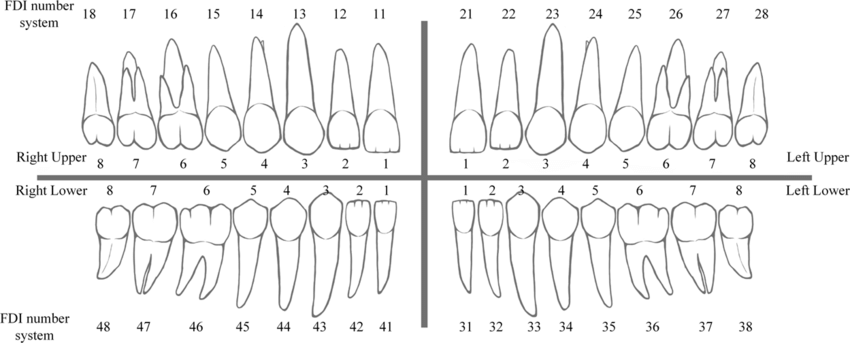
\includegraphics[width=\linewidth]{Prilohy/Obrazky/FDITeethLabels.png}
    \caption{Úkázka jednotlivých zubů s příslušným označením v podobě čísel jdoucím po směru hodinových ručiček. (převzato z \cite{teethLabelImg})}
    \label{fig:teethLabel}
\end{figure}

Pro lepší orientaci je ústní dutina rozdělena do čtyř kvadrantů a zuby jsou označeny ve směru hodinových ručiček dvojčíslím, kde první číslo označuje číslo zubu a druhé kvadrant, ve kterém se zub nachází viz \ref{fig:teethLabel}. Toto označení zubů se nazývá FDI \cite{FDI-teeth_labeling} a zahrnuje všechny důležité informace, což usnadňuje přesné a konzistentní anotování.

\subsection{Aplikace šumu na snímky v datové sadě}
Následující sekce je soustředěna na přidávání šumu do snímků ve vytvořené datové sadě, aby bylo možné vytvořit trénovací a validační sady pro vyhodnocování algoritmů redukce šumu. V první kapitole byly popsány nejčastěji se vyskytující typy šumu ve snímcích. V této práci se zaměřím na redukci tří nejčastějších typů šumů v rentgenových snímcích: speckle šum, impulzní šum a Poissonův šum \cite{MostCommonNoises}.

Ve vytvořené datové sadě se nachází 5000 rentgenů hrudníku a 500 rentgenů zubů. Na snímky budou aplikovány zmíněné typy šumů následovně:

\begin{table}[h]
    \centering
    \begin{tabular}{|l|l|}
        \hline
        \textbf{Část datasetu v \%} & \textbf{Typ aplikovaného šumu}                    \\ \hline
        0-20   & Na snímky v tomto rozsahu bude aplikován šum typu speckle.             \\ \hline
        20-40  & Tato část bude ovlivněna typem šumu soli a pepře.                      \\ \hline
        40-60  & Tento rozsah bude zašuměn Poissonův šumem.                             \\ \hline
        60-80  & Zde bude aplikována náhodná kombinace dvou typů šumu.                  \\ \hline
        80-100 & Poslední část snímků bude zašuměna všemi třemi typy šumu.              \\ 
        \hline
    \end{tabular}
    \caption{Detailní popis aplikace šumu na snímky v datové sadě}
    \label{table:noiseTypes}
\end{table}

Tento postup umožňuje vytvoření různých úrovní obtížnosti při odstraňování šumu, což je klíčové pro vývoj a vyhodnocení robustních modelů pro redukci šumu.

Nejprve jsem aplikoval jednotlivé typy šumů samostatně na části datasetu (první tři řádky v tabulce \ref{table:noiseTypes}), což vytváří relativně jednoduše odstranitelné šumové artefakty. Tímto způsobem můžu zhodnotit základní schopnosti algoritmů pro redukci šumu efektivně odstraňovat každý typ šumu zvlášť. Čtvrtý řádek v tabulce \ref{table:noiseTypes} představuje střední úroveň obtížnosti. Tento krok testuje algoritmy v situacích, kde musí řešit více šumových podmínek současně, což simuluje složitější a realističtější scénáře, jaké mohou nastat v praxi. Poslední řádek tabulky \ref{table:noiseTypes} odpovídá nejnáročnějším scénářům pro vytvořené algoritmy, které musí být schopny odstranit kombinaci různých typů šumů. Tyto snímky jsou klíčové pro testování a vývoj velmi robustních modelů, které mohou efektivně fungovat v nejrůznějších reálných situacích.

Tento stratifikovaný přístup k aplikaci šumu nejen zajišťuje důkladné testování algoritmů pro redukci šumu ve snímcích, ale také pomáhá při vývoji a ladění modelů, které jsou schopny se přizpůsobit různým úrovním šumové zátěže. Tímto způsobem dosáhnu komplexního hodnocení technik pro zpracování rentgenových snímků v různých podmínkách.

\subsubsection{Měření hodnoty šumu ve snímcích}
Pro aplikaci šumu na snímky jsem využil knihovnu \texttt{numpy} \cite{Numpy}, se kterou jsem implementoval funkce pro přidání speckle šumu, šumu soli a pepře a Poissonova šumu. Hlavním parametrem těchto funkcí je intenzita šumu, nikoli jeho směrodatná odchylka (std). Použití intenzity jako parametru je praktické pro aplikaci různých úrovní šumu, ale pro analýzu a srovnání je často nutné znát skutečnou směrodatnou odchylku šumu v obraze. Proto jsem vyvinul následující funkci, která odhaduje směrodatnou odchylku šumu v obraze pomocí extrakce segmentů (anglicky "patches") a analýzy hlavních komponent (PCA). Následující kód ukazuje implementaci zmíněné funkce\footnote{Kompletní implementace funkcí pro přidání šumu lze nalézt v GitHub repozitáři této práce.}.

\begin{lstlisting}[language=Python, caption={Funkce pro odhad směrodatné odchylky šumu ve snímku}, label={lst:noise_estimation}]
    import numpy as np
    from sklearn.feature_extraction.image import extract_patches_2d
    from sklearn.decomposition import PCA
    from typing import Tuple

    def estimate_noise_in_image(
        image: np.ndarray, patch_size: Tuple[int, int] = (7, 7), num_patches: int = 1000,
        lower_percentile: float = 0.1, upper_percentile: float = 0.2
    ) -> tuple:
        (*\# Extrahuje segmenty *)
        patches = extract_patches_2d(image, patch_size, max_patches=num_patches)
        
        (*\# Přetvoří segmenty na 2D pole, kde každý řádek je segment *)
        patches = patches.reshape(patches.shape[0], -1).astype(np.float32)
        
        (*\# Odebere průměr *)
        patches -= np.mean(patches, axis=1, keepdims=True)
        
        (*\# PCA pro nalezení vlastních čísel *)
        pca = PCA(n_components=patch_size[0]*patch_size[1])
        pca.fit(patches)
        
        (*\# Vypočítá indexy pro požadovaný percentilní v rozsahu vlastních čísel *)
        lower_index = int(lower_percentile * len(pca.explained_variance_))
        upper_index = int(upper_percentile * len(pca.explained_variance_))
        
        (*\# Medián vlastních čísel ve specifikovaném percentilním rozsahu *)
        noise_variance = np.median(pca.explained_variance_[lower_index:upper_index])
        
        return np.sqrt(pca.explained_variance_), np.sqrt(noise_variance)
\end{lstlisting}

Tato funkce mi umožňuje kvantifikovat a porovnávat úrovně šumu a pomocí těchto odhadů mohu lépe analyzovat výkon algoritmů na různých úrovních šumu. Pro ukázku výstupu z popsané metody slouží následující graf \ref{fig:PCA_std}, na kterém je zobrazena hodnota směrodatné odchylky šumu na daném snímku. Na tento snímek, byla aplikována kombinace tří různých typů šumů a jedná se tedy o silně zašuměný snímek. Hodnota směrodatné odchylky se v grafu pohybuje v rozmezí od 80 do 50. Jelikož hodnota směrodatné odchylky u čistých snímků dosahuje maximálně hodnoty 20, je zřejmé, že se skutečně jedná o silně degradovaný snímek.

\begin{figure}[h]
    \centering
    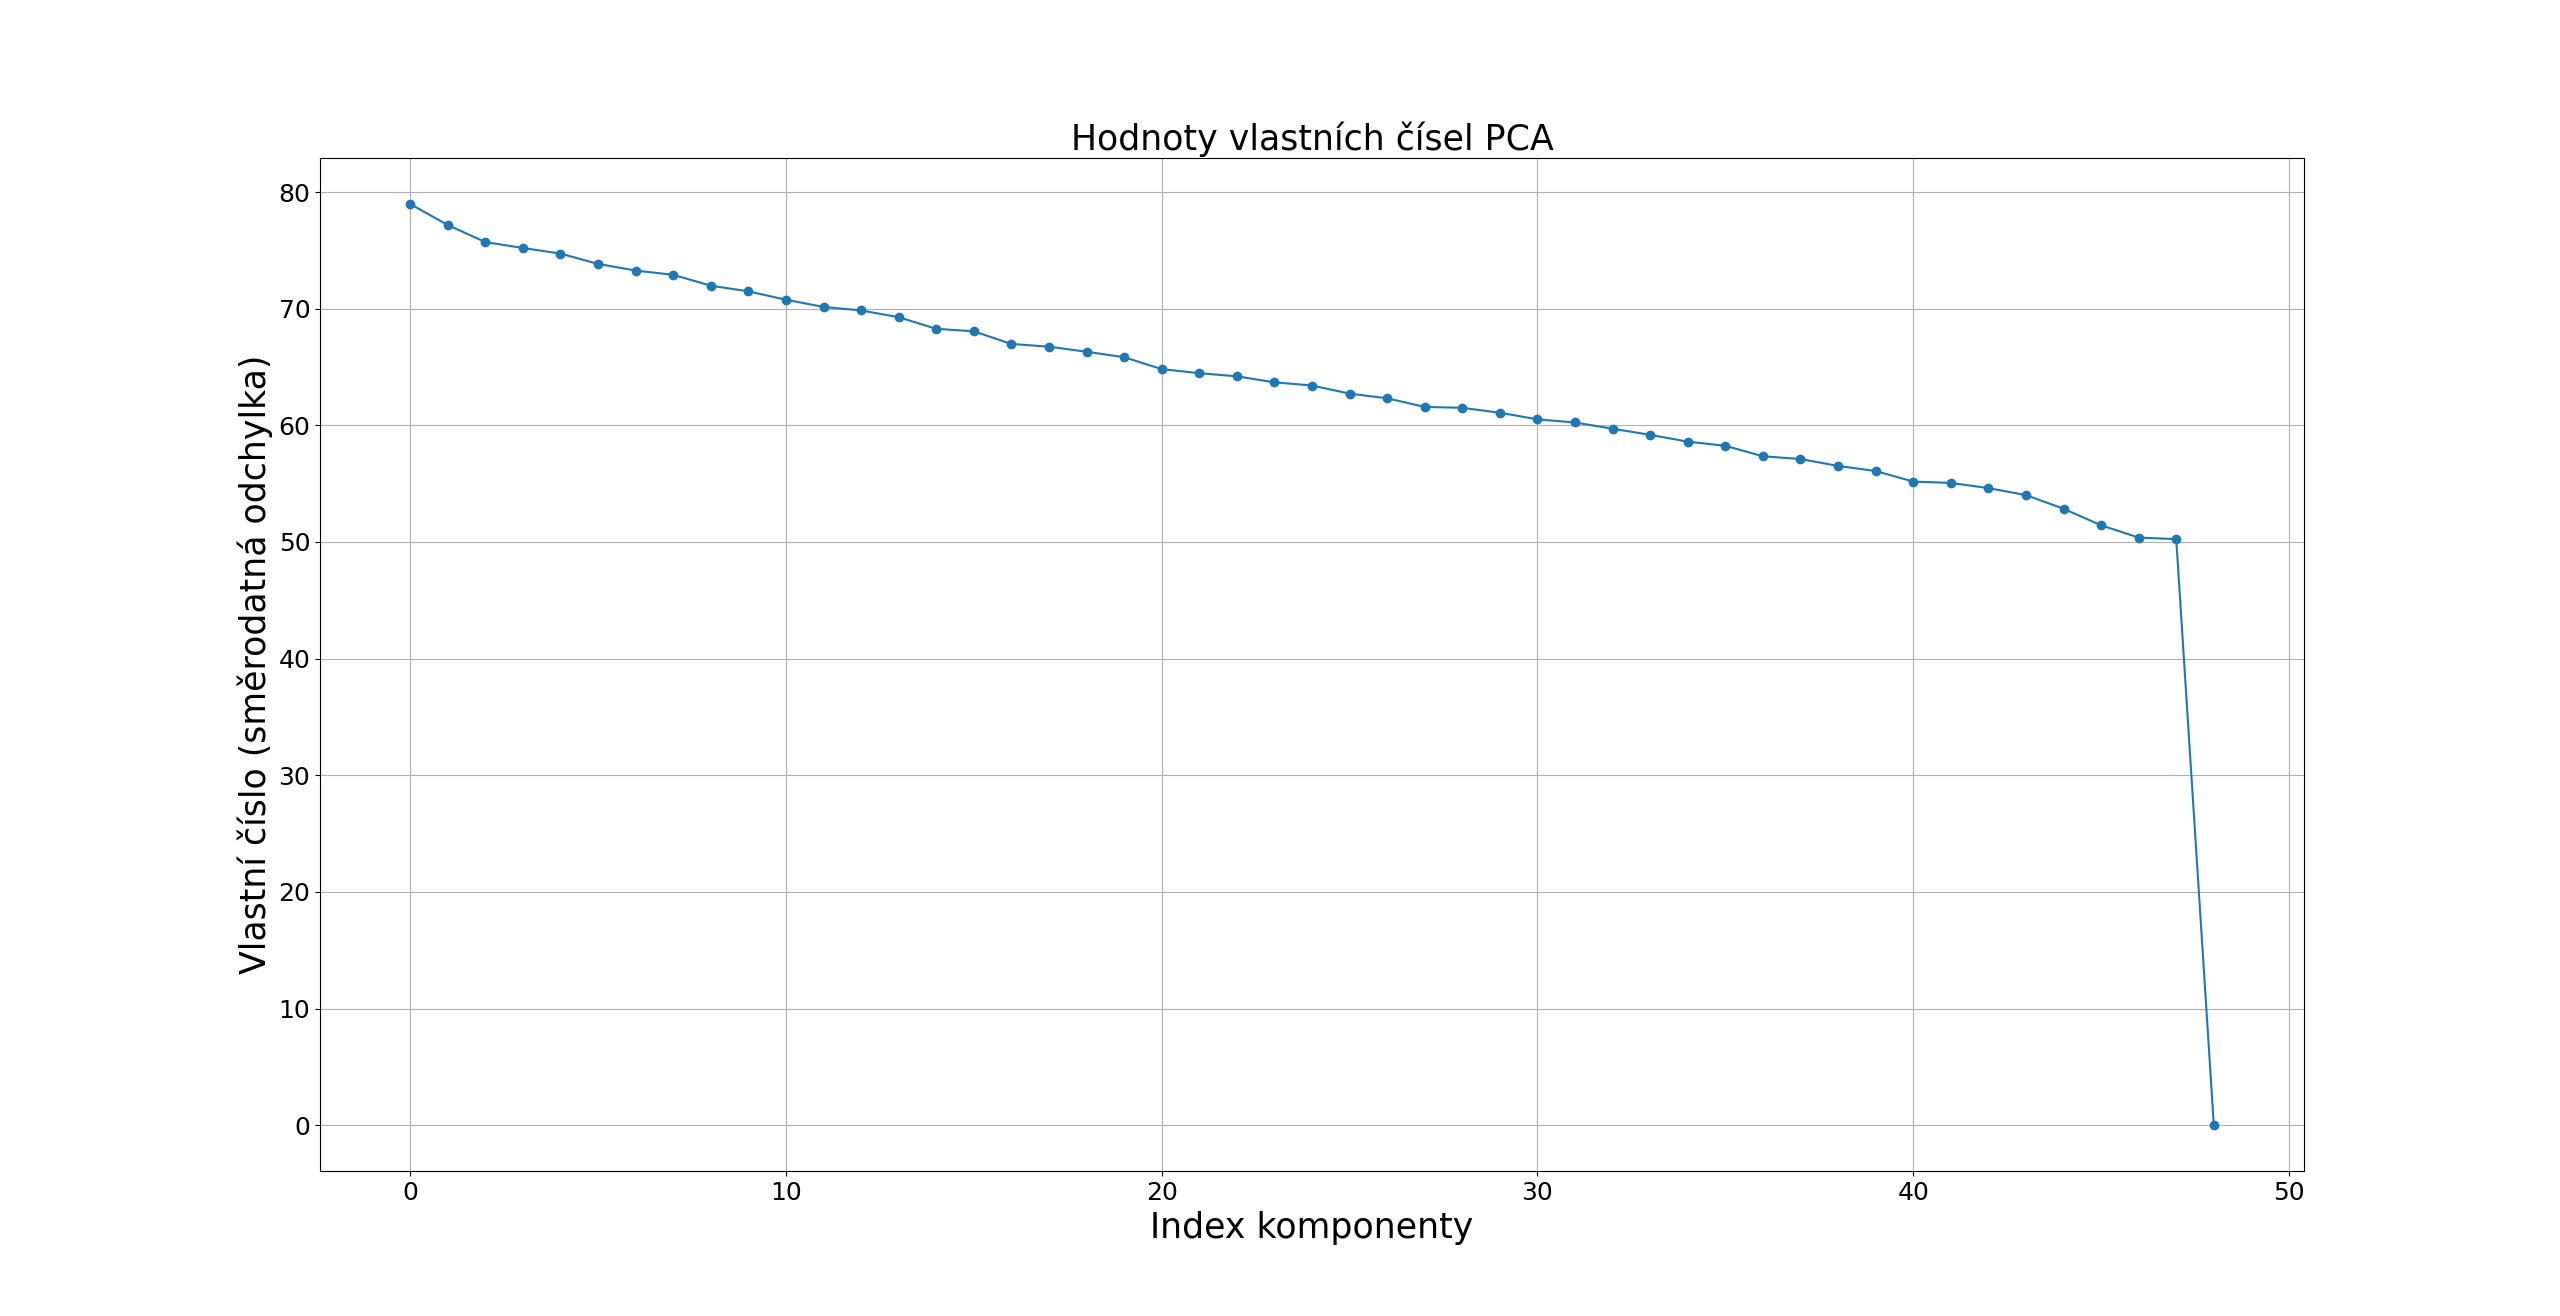
\includegraphics[width=\linewidth]{Prilohy/Obrazky/PCA_std_all_three_noise_types.png}
    \caption{Graf zobrazující hodnotu směrodatné odchylky silně zašuměného snímku.}
    \label{fig:PCA_std}
\end{figure}

\section{Návrh metod vhodných pro předzpracování rentgenových snímků}
V této části se budu zabývat charakteristikou použitých knihoven a technologií, nastavením projektu pomocí nástroje Poetry \cite{Poetry} a implementací různých standardních metod používaných pro odstranění šumu a zlepšení kvality obrazu. Zatímco teoretické pozadí a principy těchto metod byly popsány v teoretické části této práce, následující část se zaměřuje na praktické aspekty jejich implementace, včetně jakýchkoliv dalších algoritmů, které dosud nebyly zmíněny. Dále vysvětlím použití tzv. \textit{Ensemble Averaging} postupu \cite{EnsembleAveraging}, který napomáhá ke zlepšení robustnosti algoritmů pro redukci šumu.

\subsection{Struktura projektu, použité knihovny a technologie}
Pro tento projekt jsem zvolil nástroj Poetry, který umožňuje snadnou správu závislostí a vytváření virtuálních prostředí. Poetry poskytuje pohodlný způsob, jak udržovat konzistenci balíčků a odděluje závislosti projektu od systémových knihoven. To usnadňuje sdílení projektu a zajišťuje, že všechny potřebné knihovny budou správně nainstalovány.

\subsubsection{Instalace a konfigurace Poetry}
Instalace nástroje Poetry začíná instalací pipx, což je nástroj umožňující instalaci a izolaci Python aplikací. 

\begin{lstlisting}[language=bash, caption={Instalace pipx}]
    python -m pip install pipx
\end{lstlisting}

Poté pomocí pipx je možné nainstalovat nástroj Poetry:

\begin{lstlisting}[language=bash, caption={Instalace Poetry}]
    pipx install poetry
\end{lstlisting}

Po instalaci Poetry je nutné se přesunout do kořenového adresáře projektu a nainstalovat všechny závislosti definované v souboru pyproject.toml pomocí následujícího příkazu:

\begin{lstlisting}[language=bash, caption={Instalace virtuálního prostředí a knihoven}]
    cd cesta/k/projektu
    poetry install
\end{lstlisting}

\subsubsection{Použité knihovny}
V tomto projektu jsem použil několik důležitých knihoven. Nejvýznamnější z nich je \textbf{PyTorch Lightning} \cite{Pytorchlightning}, která usnadňuje implementaci neuronových sítí a byla vybrána pro snadné a přehledné trénování modelů. Další důležité knihovny zahrnují již dříve zmíněný NumPy pro numerické výpočty, scikit-image \cite{Scikit} pro zpracování snímků a Matplotlib \cite{Matplotlib} pro vizualizaci dat. Následující tabulka ukazuje kompletní přehled použitých závislostí v této práci:

\begin{table}[h]
    \centering
    \begin{tabular}{|l|l|}
    \hline
    \textbf{Knihovna}       & \textbf{Popis}                                          \\ \hline
    \textbf{python}         & Základní programovací jazyk pro tento projekt.          \\ \hline
    \textbf{torch}          & Hlavní knihovna pro implementaci neuronových sítí.      \\ \hline
    \textbf{torchaudio}     & Knihovna pro zpracování audio dat v PyTorch.            \\ \hline
    \textbf{torchvision}    & Knihovna pro zpracování obrazových dat v PyTorch.       \\ \hline
    \textbf{lightning}      & Framework pro snadné trénování modelů v PyTorch.        \\ \hline
    \textbf{pillow}         & Knihovna pro práci s obrazovými daty.                   \\ \hline
    \textbf{pandas}         & Knihovna pro manipulaci s daty a jejich analýzu.        \\ \hline
    \textbf{pydantic}       & Knihovna pro validaci dat.                              \\ \hline
    \textbf{opencv-python}  & Knihovna pro práci s obrazovými daty a předzpracování.  \\ \hline
    \textbf{torchmetrics}   & Knihovna pro výpočet metrik pro hodnocení modelů.       \\ \hline
    \textbf{matplotlib}     & Knihovna pro vizualizaci dat.                           \\ \hline
    \textbf{mlflow}         & Nástroj pro sledování experimentů a modelů.             \\ \hline
    \textbf{scikit-image}   & Knihovna pro zpracování snímků.                         \\ \hline
    \textbf{rich}           & Knihovna pro pokročilé logování.                        \\ \hline
    \textbf{pywavelets}     & Knihovna pro práci s vlnkovou transformací.             \\ \hline
    \textbf{numba}          & Knihovna pro akceleraci numerických výpočtů.            \\ \hline
    \end{tabular}
    \caption{Přehled použitých nástrojů}
    \label{tab:Used_libs}
\end{table}

\subsubsection{Struktura projektu}
Projekt je strukturován tak, aby umožňoval efektivní správu kódu a snadnou navigaci mezi různými částmi. V kořenovém adresáři projektu se nachází hlavní soubor \textbf{main.py}, který zahrnuje všechny funkce pro trénování, testování a tvorbu datasetů. Složka \textbf{common} obsahuje skripty pro vizualizaci, tvorbu datasetů a základní struktury tříd. Konfigurační soubory pro různé experimenty a nastavení filtrů jsou umístěny ve složce \textbf{configs}. Předzpracování dat, jak pomocí standardních metod, tak pomocí neuronových sítí, se nachází ve složce \textbf{preprocessing}. Implementace U-Net modelu a související skripty jsou umístěny ve složce \textbf{unet}. Tento strukturovaný přístup umožňuje udržovat kód přehledný a organizovaný, což je klíčové pro efektivní vývoj.

\subsection{Vybrané metody a jejich implementace}
V této práci jsem se zaměřil na implementaci vybraných standardních metod pro odstranění šumu a zvýšení kvality obrazu. V následujícím seznamu jsou uvedeny použité metody spolu s jejich krátkým popisem: 

\begin{itemize}
    \item \textbf{CLAHE:} Zvyšuje lokální kontrast a zabraňuje nadměrnému zesílení šumu.
    \item \textbf{Mediánový Filtr:} Odstraňuje impulzní šum nahrazením každého pixelu mediánem jeho okolí.
    \item \textbf{Bilaterální Filtr:} Zachovává hrany při redukci šumu zohledněním prostorových i intenzitních rozdílů.
    \item \textbf{Filtr ne-lokálních průměrů:} Redukuje šum průměrováním podobných segmentů v celém obraze.
    \item \textbf{Lokálně adaptivní mediánový filtr:} Adaptivní mediánový filtr, který přizpůsobuje prahovou hodnotu šumu na základě místní variance.
    \item \textbf{Redukce šumu pomocí vlnkové transformace:} Rozkládá obraz na vlnkové koeficienty a odstraňuje šum pomocí prahování.
\end{itemize}

Většina uvedených metod byla implementována s využitím knihoven \texttt{scipy} \cite{scipy} a \texttt{skimage} \cite{scikit}, které poskytují optimalizované a efektivní řešení. Vzhledem k tomu, že dataset obsahuje 5500 snímků, je výpočetní efektivita klíčová pro zpracování v rozumném čase.

Některé z metod nebyly ve zmíněných knihovnách dostupné, bylo proto nutné je implementovat svépomocí. Jedná se o adaptivní mediánový filtr a Frost filtr \cite{FrostFilter}. Tyto metody jsem se snažil navrhnout tak, aby byly efektivní a rychlé, zejména Frost filtr bylo nutné implementovat s využitím knihovny \texttt{numba} \cite{numba}, která umožňuje provádět náročné výpočty na grafické kartě, což výrazně zrychlilo zpracování. Níže je uveden příklad implementace Frostova filtru:

\begin{lstlisting}[language=Python, caption={Implementace Frost filtru s využitím Numba CUDA}, label={lst:frost_filter}]
    @numba.jit(nopython=True)
    def __compute_weights(
        patch: npt.NDArray, N: int, initial_K: float, local_mean: np.float64, local_std: np.float64
    ) -> npt.NDArray[np.float64]:
        center_pixel = patch[N, N]
        T_t0 = np.abs(center_pixel - local_mean) / local_std if local_std != 0 else 0
        weights = np.zeros_like(patch)
    
        for i in range(patch.shape[0]):
            for j in range(patch.shape[1]):
                current_pixel = patch[i, j]
                numerator = np.abs(current_pixel - center_pixel)
                abs_diffs = np.abs(patch - center_pixel)
                abs_diffs[N, N] = 0  # Exclude the center pixel from the sum
                total_pixels = (2 * N + 1) ** 2 - 1
                denominator = np.sum(abs_diffs) / total_pixels
                Q_sh = numerator / denominator if denominator != 0 else 0
                K = initial_K * T_t0 * Q_sh
                d_sh = np.sqrt((i - N) ** 2 + (j - N) ** 2)
                weights[i, j] = np.exp(-K * d_sh)
        
        return weights
    
    
    def apply_frost_filter(
        image: npt.NDArray, window_size: int = 3, initial_K: float = 1.0
    ) -> npt.NDArray:
        def adaptive_kernel(patch: npt.NDArray) -> np.float64:
            patch = patch.reshape(window_size, window_size)
            N = window_size // 2
            local_mean = np.mean(patch)
            local_std = np.std(patch)
            weights = __compute_weights(patch, N, initial_K, local_mean, local_std)
            weights /= np.sum(weights)
            return np.sum(weights * patch)
    
        filtered_image = generic_filter(image, adaptive_kernel, size=(window_size, window_size))
        filtered_image_uint8 = np.clip(filtered_image, 0, 255).astype(np.uint8)
        return filtered_image_uint8
\end{lstlisting}

\subsection{Ensemble averaging}
Vzhledem k omezením standardních metod pro odstranění šumu, jsem se rozhodl implementovat přístup zvaný ensemble averaging. Tento přístup kombinuje výsledky několika různých metod pro odstranění šumu a poskytuje tak robustnější a efektivnější řešení.

Hlavním důvodem pro použití ensemble averaging je překonání omezení jednotlivých metod. Jak již bylo zmíněno, každá standardní metoda má své silné a slabé stránky, a samotné použití jedné metody nemusí být dostatečné pro dosažení optimálních výsledků v reálných scénářích, kde může být přítomno více typů šumu.

Ensemble averaging využívá kombinaci několika metod k dosažení následujících výhod:

\begin{itemize}
    \item \textbf{Robustnost:} Kombinací výsledků z různých metod lze dosáhnout robustnějšího odstranění šumu, které není závislé na jednom specifickém typu šumu.
    \item \textbf{Zlepšení kvality obrazu:} Průměrováním výsledků se minimalizují chyby a artefakty, které mohou vzniknout při použití jednotlivých metod.
    \item \textbf{Přizpůsobivost:} Tento přístup je přizpůsobivý různým typům šumu a jejich kombinacím, což je klíčové pro praktické aplikace.
\end{itemize}

Implementace ensemble averaging zahrnuje několik kroků. Každý obraz je zpracován několika různými metodami pro odstranění šumu, které jsou aplikovány samostatně, aby se zabránilo vzájemnému ovlivňování. Výstupy těchto metod jsou poté průměrovány za účelem vytvoření finálního obrazu s odstraněným šumem. Níže je ukázka kódu pro implementaci ensemble averaging:

\begin{lstlisting}[language=Python, caption={Implementace Ensemble Averaging metody}, label={lst:ensemble_averaging}]
    def apply_standard_preprocessing(
        image: npt.NDArray, transform_type: str, params: Dict | None = None
    ) -> Image.Image:
        preprocessing_method = getattr(standart_preprocessing, f"apply_{transform_type}")

        if preprocessing_method and callable(preprocessing_method):
            if params is None:
                return Image.fromarray(preprocessing_method(image))
            else:
                return Image.fromarray(preprocessing_method(image, **params))
        else:
            print("No preprocessing was applied!")
            return Image.fromarray(image)


    def standard_preprocessing_ensemble_averaging(
        image: npt.NDArray[np.uint8], preprocessing_config: Dict[str, Dict[str, Any]]
    ) -> Image.Image:
        preprocessed_images: List[npt.NDArray[np.float64]] = []

        for method, params in track(
            sequence=preprocessing_config.items(),
            description="Applying preprocessing method...",
            total=len(preprocessing_config),
        ):
            image_copy = np.array(image, copy=True)
            processed_image = apply_standard_preprocessing(image_copy, method, params)
            preprocessed_images.append(np.array(processed_image))

        averaged_image = cast(npt.NDArray[np.float64], np.mean(preprocessed_images, axis=0))
        return Image.fromarray(averaged_image.astype(np.uint8))
\end{lstlisting}

Ensemble averaging nabízí několik výhod, které zlepšují kvalitu výsledného obrazu a jeho robustnost. Kombinace výsledků z různých metod pro odstranění šumu vede k lepšímu celkovému odstranění šumu, protože silné stránky jednotlivých metod se navzájem doplňují. Tento přístup zajišťuje, že výsledný obraz je méně náchylný k artefaktům a chybám, které mohou vzniknout při použití pouze jedné metody. Díky tomu je možné dosáhnout vyšší kvality obrazu, a to i v přítomnosti různých typů šumu.

Nicméně ensemble averaging má také svá omezení. Jedním z hlavních problémů je výpočetní náročnost, protože každá metoda musí být aplikována samostatně na každý obraz, což výrazně zvyšuje dobu zpracování. Dalším omezením je složitost nastavení parametrů jednotlivých metod, protože různé snímky se mohou lišit a metody mohou vykazovat odlišné chování v závislosti na těchto rozdílech. Navíc kvalita výsledného obrazu závisí na výkonnosti jednotlivých metod, pokud tedy některá metoda selže, může to negativně ovlivnit celkový výsledek.

\section{Návrh a implementace specializovaných modelů neuronových sítí}
Následující sekce bude věnována návrhu a implementaci specializovaných modelů neuronových sítí pro odstranění šumu z rentgenových snímků. Sekce bude zahrnovat detailní popis dvou různých modelů neuronových sítí: konvoluční neuronová síť pro redukci šumu (Denoising convolutional neural network DnCNN) a autoenkodér pro redukci šumu (Denoising autoencoder DAE). Popis modelů bude obsahovat podrobnosti o tom, jak jednotlivé modely fungují a bude také podrobně popsána jejich implementace, s důrazem na výsledky dosažené při odstraňování šumu.

\subsection{Neuronová síť DnCNN}
Konvoluční neuronová síť pro redukci šumu (DnCNN) je pokročilý model, který se na rozdíl od tradičních metod zaměřuje na předvídání šumu přítomného v obraze, aniž by předvídal celý obraz. Tento nalezený šum je poté odečten od zašuměného vstupu, aby se získal čistý obraz. Tato metoda využívá residuální učení (residual learning), které umožňuje síti naučit se mapování ze zašuměného obrazu na samostatný šum. Koncept a implementace DnCNN byly představeny v článku "Beyond a Gaussian Denoiser: Residual Learning of Deep CNN for Image Denoising" \cite{DnCNN}.

\subsubsection{Architektura DnCNN}
Architektura DnCNN se skládá z několika konvolučních vrstev propojených aktivačními funkcemi ReLU a normalizačními vrstvami BatchNorm. Počáteční vrstva transformuje vstupní obraz na reprezentaci do vyšší dimenze. Následuje série vrstev, z nichž každá je následována vrstvou BatchNorm a aktivační funkcí ReLU. Tyto mezivrstvy umožňují modelu efektivně extrahovat rysy z obrazu a učit se složité vzory šumu. Poslední vrstvou je konvoluční vrstva, která předpovídá šum v obraze. Síť se může zaměřit na zachycení vysokofrekvenčních složek šumu, jejichž modelování je často náročnější. Tato konstrukce výrazně zlepšuje schopnost sítě odstraňovat z obrazu různé typy šumu, což vede k lepšímu výkonu ve srovnání s běžnými metodami. Níže je implementace této architektury:

\begin{lstlisting}[language=Python, caption={Implementace konvoluční neuronové sítě pro redukci šumu}, label={lst:DnCNN}]
    import torch
    import torch.nn as nn
    from torchmetrics import MetricCollection
    from preprocessing.neural_networks.model import PreprocessingModel
    
    class DnCNN(PreprocessingModel):
        def __init__(
            self,
            depth: int = 17,
            n_channels: int = 64,
            image_channels: int = 1,
            learning_rate: float = 1e-4,
            metrics: MetricCollection | None = None,
        ) -> None:
            super(DnCNN, self).__init__(learning_rate=learning_rate, metrics=metrics)
            layers = [
                nn.Conv2d(image_channels, n_channels, kernel_size=3, padding=1),
                nn.ReLU(inplace=True),
            ]
    
            for _ in range(depth - 2):
                layers.append(nn.Conv2d(n_channels, n_channels, kernel_size=3, padding=1))
                layers.append(nn.BatchNorm2d(n_channels))
                layers.append(nn.ReLU(inplace=True))
    
            layers.append(nn.Conv2d(n_channels, image_channels, kernel_size=3, padding=1))
    
            self.dncnn = nn.Sequential((**layers*))
    
            def forward(self, x: torch.Tensor) -> torch.Tensor:
                predicted_noise = self.dncnn(x)
                return x - predicted_noise
\end{lstlisting}

\subsubsection{Tréninkový proces}
Tréninkový proces DnCNN zahrnuje několik klíčových kroků, které zajišťují, že se model efektivně naučí předvídat a odstraňovat šum ze snímků. Tento proces využívá ztrátovou funkci střední kvadratické chyby (MSE) k měření rozdílu mezi předpokládaným šumem a skutečným šumem přítomným ve snímcích.

Níže je implementace třídy PreprocessingModel, která slouží jako základní třída pro modely redukující šum, včetně DnCNN. Tato třída definuje metody pro konfiguraci optimalizátoru, pro učení a testování spolu s metrikami pro ohodnocení modelu.

\begin{lstlisting}[language=Python, caption={Třída pro model redukující šum}, label={lst:PreprocessingClass}]
    from abc import ABC, abstractmethod
    from typing import Any, Dict
    import torch
    import torch.nn.functional as F
    import torch.optim as optim
    from lightning import LightningModule
    from torchmetrics import MeanSquaredError, MetricCollection

    class PreprocessingModel(LightningModule, ABC):
        def __init__(
            self,
            learning_rate: float = 1e-4,
            metrics: MetricCollection | None = None,
        ) -> None:
            super(PreprocessingModel, self).__init__()
            self.learning_rate = learning_rate
            self.metrics = metrics or MetricCollection({"MSE": MeanSquaredError()})
            self.save_hyperparameters(ignore=["metrics"])

        @abstractmethod
        def forward(self, x: torch.Tensor) -> torch.Tensor:
            pass

        def configure_optimizers(self) -> Dict[str, Any]:
            optimizer = optim.Adam(self.parameters(), lr=self.learning_rate)
            return {"optimizer": optimizer}

        def training_step(
            self, batch: Any, batch_idx: int
        ) -> torch.Tensor:
            noised_images, target = batch
            denoised_images = self(noised_images)
            loss = F.mse_loss(denoised_images, target)
            self.log("train_loss", loss, on_step=True, prog_bar=True, logger=True)
            return loss

        def validation_step(
            self, batch: Any, batch_idx: int
        ) -> None:
            noised_images, target = batch
            denoised_images = self(noised_images)

            loss = F.mse_loss(denoised_images, target)
            self.log("val_loss", loss, on_epoch=True, prog_bar=True, logger=True)
            self.log_metrics(denoised_images, target)

        def log_metrics(
            self, denoised_images, target
        ) -> None:
            metrics: Dict[str, Any] = self.metrics(denoised_images, target)
            for name, value in metrics.items():
                self.log(f"val_{name}", value)
\end{lstlisting}

Tato třída slouží jako základ pro model DnCNN, který tuto třídu zdědí, implementuje specifickou architekturu a dopředný průchod pro predikci šumu.

\subsection{Návrh autoenkodéru pro redukci šumu}
Autoenkodér pro redukci šumu (DAE) je model hlubokého učení navržený k redukci šumu ze snímků předpovídáním celého čistého snímku, nikoli pouze šumu jako v případě modelu DnCNN. Tento přístup umožňuje modelu naučit se komplexní vztahy v daném obraze, čímž může nejen efektivněji redukovat různé typy šumů, ale také vytvořit obraz věrnější svému původnímu zdrojovému snímku. DAE je složitější neuronová síť než DnCNN, protože obsahuje více vrstev a neuronů, což by mělo přispět k lepší schopnosti detekce šumu. Nicméně, vytvoření robustnější sítě znamená, že model bude potřebovat větší množství tréninkových dat. Jejich nedostatek může vést k tomu, že se model začne přizpůsobovat specifikám tréninkových dat a může ztrácet na obecném výkonu.

\subsubsection{Architektura DAE}
Architektura DAE se skládá ze dvou hlavních součástí: enkodéru a dekodéru. Obě části jsou konstruovány pomocí konvolučních a dekonvolučních vrstev s aktivačními funkcemi ReLU a batch normalizací. Enkodér i dekodér obsahují každý šest vrstev, přičemž každá vrstva je navržena tak, aby postupně zpracovávala obrazové informace a detekovala složitější vzory ve snímcích.

Enkodér komprimuje vstupní obraz do nižší dimenzionální reprezentace pomocí postupně aplikovaných konvolučních vrstev. Každá vrstva extrahuje stále složitější rysy z obrazových dat. Dekodér rekonstruuje čistý obraz z komprimované reprezentace využitím dekonvolučních vrstev. Vrstvy dekodéru postupně zvětšují rozlišení a kombinují informace z enkodéru pomocí tzv. \textit{skip connections}. Skip connections umožňují přenášet informace z odpovídajících vrstev enkodéru přímo do dekodéru, čímž napomáhají zachovat prostorové detaily a rysy z původního obrazu, které by mohly být ztraceny během komprimace.

Architektura DAE je detailně znázorněna na diagramu \ref{fig:DAE}. Diagram ilustruje, jak jsou jednotlivé vrstvy enkodéru a dekodéru propojeny a také znázorňuje předávání dodatečných informací prostřednictvím skip connections. Enkodér začíná s konvoluční vrstvou s 64 filtry a postupně zvyšuje počet filtrů až na 512, zatímco dekodér postupně generuje obraz zpět do jeho původního rozlišení pomocí dekonvolučních vrstev. Níže je uvedena konkrétní implementace tříd autoenkodéru pro redukci šumu.

\begin{lstlisting}[language=Python, caption={Implementace autoenkodéru pro redukci šumu}, label={lst:DAEClass}]
    import torch
    import torch.nn as nn
    from lightning import LightningModule
    from torchmetrics import MetricCollection
    from preprocessing.neural_networks.model import PreprocessingModel

    class ConvBlock(LightningModule):
        def __init__(
            self, in_channels: int, out_channels: int, kernel_size: int = 3,
            padding: int = 1, stride: int = 1,
        ) -> None:
            super(ConvBlock, self).__init__()
            self.conv = nn.Sequential(
                nn.Conv2d(
                    in_channels, out_channels, kernel_size=kernel_size,
                    padding=padding, stride=stride,
                ),
                nn.ReLU(inplace=True),
                nn.Dropout(0.2),
                nn.BatchNorm2d(out_channels),
            )

        def forward(self, x: torch.Tensor) -> torch.Tensor:
            return self.conv(x)

    class DeConvBlock(LightningModule):
        def __init__(
            self, in_channels: int, out_channels: int, kernel_size: int = 3,
            stride: int = 1, padding: int = 1, output_padding: int = 1,
        ) -> None:
            super(DeConvBlock, self).__init__()
            self.conv = nn.Sequential(
                nn.ConvTranspose2d(
                    in_channels, out_channels, kernel_size=kernel_size, stride=stride,
                    padding=padding, output_padding=output_padding,
                ),
                nn.ReLU(inplace=True),
                nn.Dropout(0.2),
                nn.BatchNorm2d(out_channels),
            )

        def forward(self, x: torch.Tensor) -> torch.Tensor:
            return self.conv(x)

    class DenoisingAutoencoder(PreprocessingModel):
        def __init__(
            self, n_channels: int = 1, learning_rate: float = 1e-4,
            metrics: MetricCollection | None = None,
        ) -> None:
            super(DenoisingAutoencoder, self).__init__(
                learning_rate=learning_rate, metrics=metrics
            )        
            self.encoder_layers = nn.ModuleList([
                ConvBlock(n_channels, 64, 3, stride=1),
                ConvBlock(64, 64, 3, stride=2),
                ConvBlock(64, 128, 5, stride=2, padding=2),
                ConvBlock(128, 128, 3, stride=1),
                ConvBlock(128, 256, 5, stride=2, padding=2),
                ConvBlock(256, 512, 3, stride=2),
            ])
            
            self.decoder_layers = nn.ModuleList([
                DeConvBlock(512, 512, 3, stride=2),
                DeConvBlock(512, 256, 3, stride=2),
                DeConvBlock(256, 128, 5, stride=2, padding=2),
                DeConvBlock(128, 64, 3, stride=2),
                DeConvBlock(64, 64, 3, stride=1, output_padding=0),
                DeConvBlock(64, n_channels, 3, output_padding=0),
            ])
            
            self.adjust_layers = nn.ModuleList([
                nn.Conv2d(768, 512, kernel_size=1),
                nn.Conv2d(384, 256, kernel_size=1),
                nn.Conv2d(192, 128, kernel_size=1),
                nn.Conv2d(128, 64, kernel_size=1),
            ])

            # Encoder layers that will be connected to decoder -> n-1
            self.skip_connection_layer_idxs = [4, 2, 1, 0]

        def forward(self, x: torch.Tensor) -> torch.Tensor:
            # Encoder
            encoder_outputs = []
            for encoder_layer in self.encoder_layers:
                x = encoder_layer(x)
                encoder_outputs.append(x)
            
            # Decoder with skip connections
            for i, decoder_layer in enumerate(self.decoder_layers):
                x = decoder_layer(x)
                if i < len(self.skip_connection_layer_idxs):
                    x = torch.cat([x, encoder_outputs[self.skip_connection_layer_idxs[i]]], dim=1)  # skip connections
                    x = self.adjust_layers[i](x)  # adjust channels
            
            return x
\end{lstlisting}

\begin{figure}[h]
    \centering
    \includegraphics[width=\linewidth]{Prilohy/Obrazky/DAE_UML.png}
    \caption{Diagram zobrazující architekturu denoising autoenkodéru.}
    \label{fig:DAE}
\end{figure}

\clearpage

\section{Výsledky standardních metod a neuronových sítí DnCNN a DAE při redukování šumu v rentgenových snímcích}
Pro vyhodnocení výkonu standardních metod a natrénovaných modelů neuronových sítí je nezbytné stanovit kvalitu samotných zašuměných snímků v porovnání s jejich originálními protějšky. Toto vyhodnocení pomáhá pochopit rozsah zlepšení dosaženého metodami a modely pro odstranění šumu. Průměrná hodnota naměřené metriky PSNR pro zašuměné snímky je zhruba 25 dB a průměrná hodnota SSIM vychází přibližně 60 \%.

\subsection{Vyhodnocení standardních metod}
Standardní metody v podobě ensemble averaging vykozovali velmi dobré výsledky při redukci Poissonova a speckle šumu. V případě šumu soli a pepře nebo kombinací šumů, ve kterých se tento šum soli a pepře vyskytoval, již metody ztráceli na účinnosti. Průměrně ensemble averaging dosáhl metriky PSNR 29 dB a metriky SSIM 85 \%, což v porovnání se zašuměnými snímky vykazuje zlepšení a použitím těchto metod vede ke zlepšení kvality daných snímků. V tabulce \ref{tab:EnsembleResults} jsou ukázány výsledky ensemble averaging pro jednotlivé typy šumů a jejich kombinací.

\begin{table}[h]
    \centering
    \begin{tabular}{|l|l|l|}
    \hline
    \textbf{Typ šumu}               & \textbf{PSNR} & \textbf{SSIM} \\ \hline
    Poissonův                       & 37 dB         &  96 \%        \\ \hline
    Speckle                         & 33 dB         &  86 \%        \\ \hline
    Sůl a pepř                      & 27 dB         &  70 \%        \\ \hline
    Poissonův, speckle              & 31 dB         &  83 \%        \\ \hline
    Poissonův, sůl a pepř           & 26 dB         &  70 \%        \\ \hline
    Speckle, sůl a pepř             & 25 dB         &  65 \%        \\ \hline
    Poissonův, speckle, sůl a pepř  & 25 dB         &  63 \%        \\ \hline
    \end{tabular}
    \caption{Ukázka výsledků kvalitu obrazu po odšumění pomocí ensemble averaging}
    \label{tab:EnsembleResults}
\end{table}

\subsection{Vyhodnocení natrénovaných modelů sítě DnCNN}
Modely trénované na architektuře DnCNN, byly velmi úspěšné při odstraňování šumu a značně vylepšily kvalitu daných rentgenových snímků. Model s nejlepšími výsledky byl trénován po dobu 55 epoch a dosáhl průměrného PSNR 31 dB a SSIM 91 \%, což ukazuje podstatné zvýšení měřených metrik jak v redukci šumu, tak ve strukturální podobnosti. Model byl trénován na snímcích z obou datových sad, protože základní charakteristiky šumu rentgenových snímků nevyžadují rozlišování mezi rentgenovými snímky plic nebo zubů. Hodnoty metrik pro jednotlivé typy šumů je možné vidět v tabulce \ref{tab:DnCNNResults}. Z výsledků je patrné, že model sítě DnCNN dokáže velmi dobře potlačit téměř všechny typy šumů, ovšem jako v případě ensemble averiging nejmenší zlepšení vykazují snímky, na které byl aplikován šum soli a pepře. Na snímcích \ref{fig:DnCNN_lungs} a \ref{fig:DnCNN_teeth} je ukázán příklad použití nejlepšího natrénovaného modelu. Ze snímků je patrné, že došlo k velmi účinné redukci šumu se zachováním podstatných detailů.

\begin{figure}[h]
    \centering
    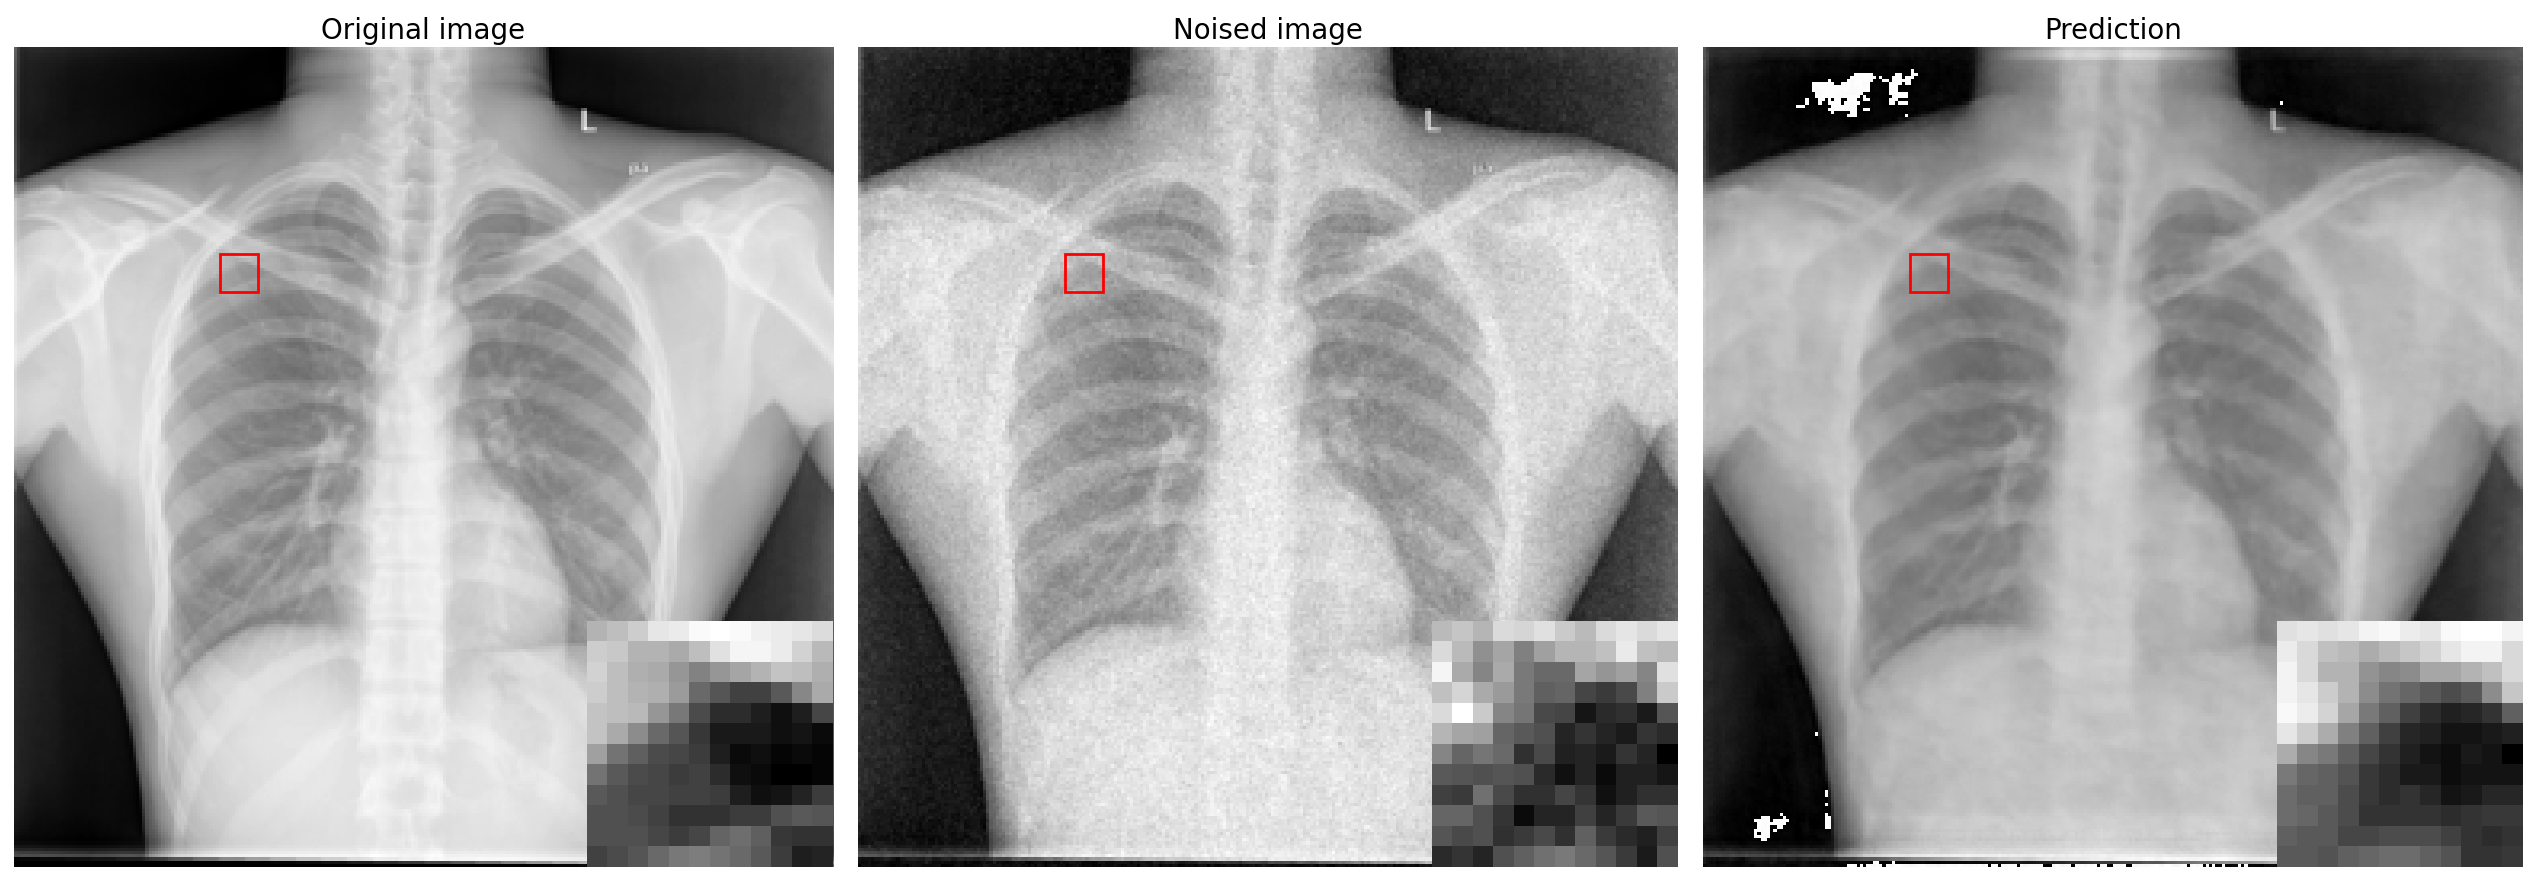
\includegraphics[width=\linewidth]{Prilohy/Obrazky/DnCNN_lungs.png}
    \caption{Ukázka odstranění šumu ze snímku plic pomocí DnCNN}
    \label{fig:DnCNN_lungs}
\end{figure}

\begin{figure}[h]
    \centering
    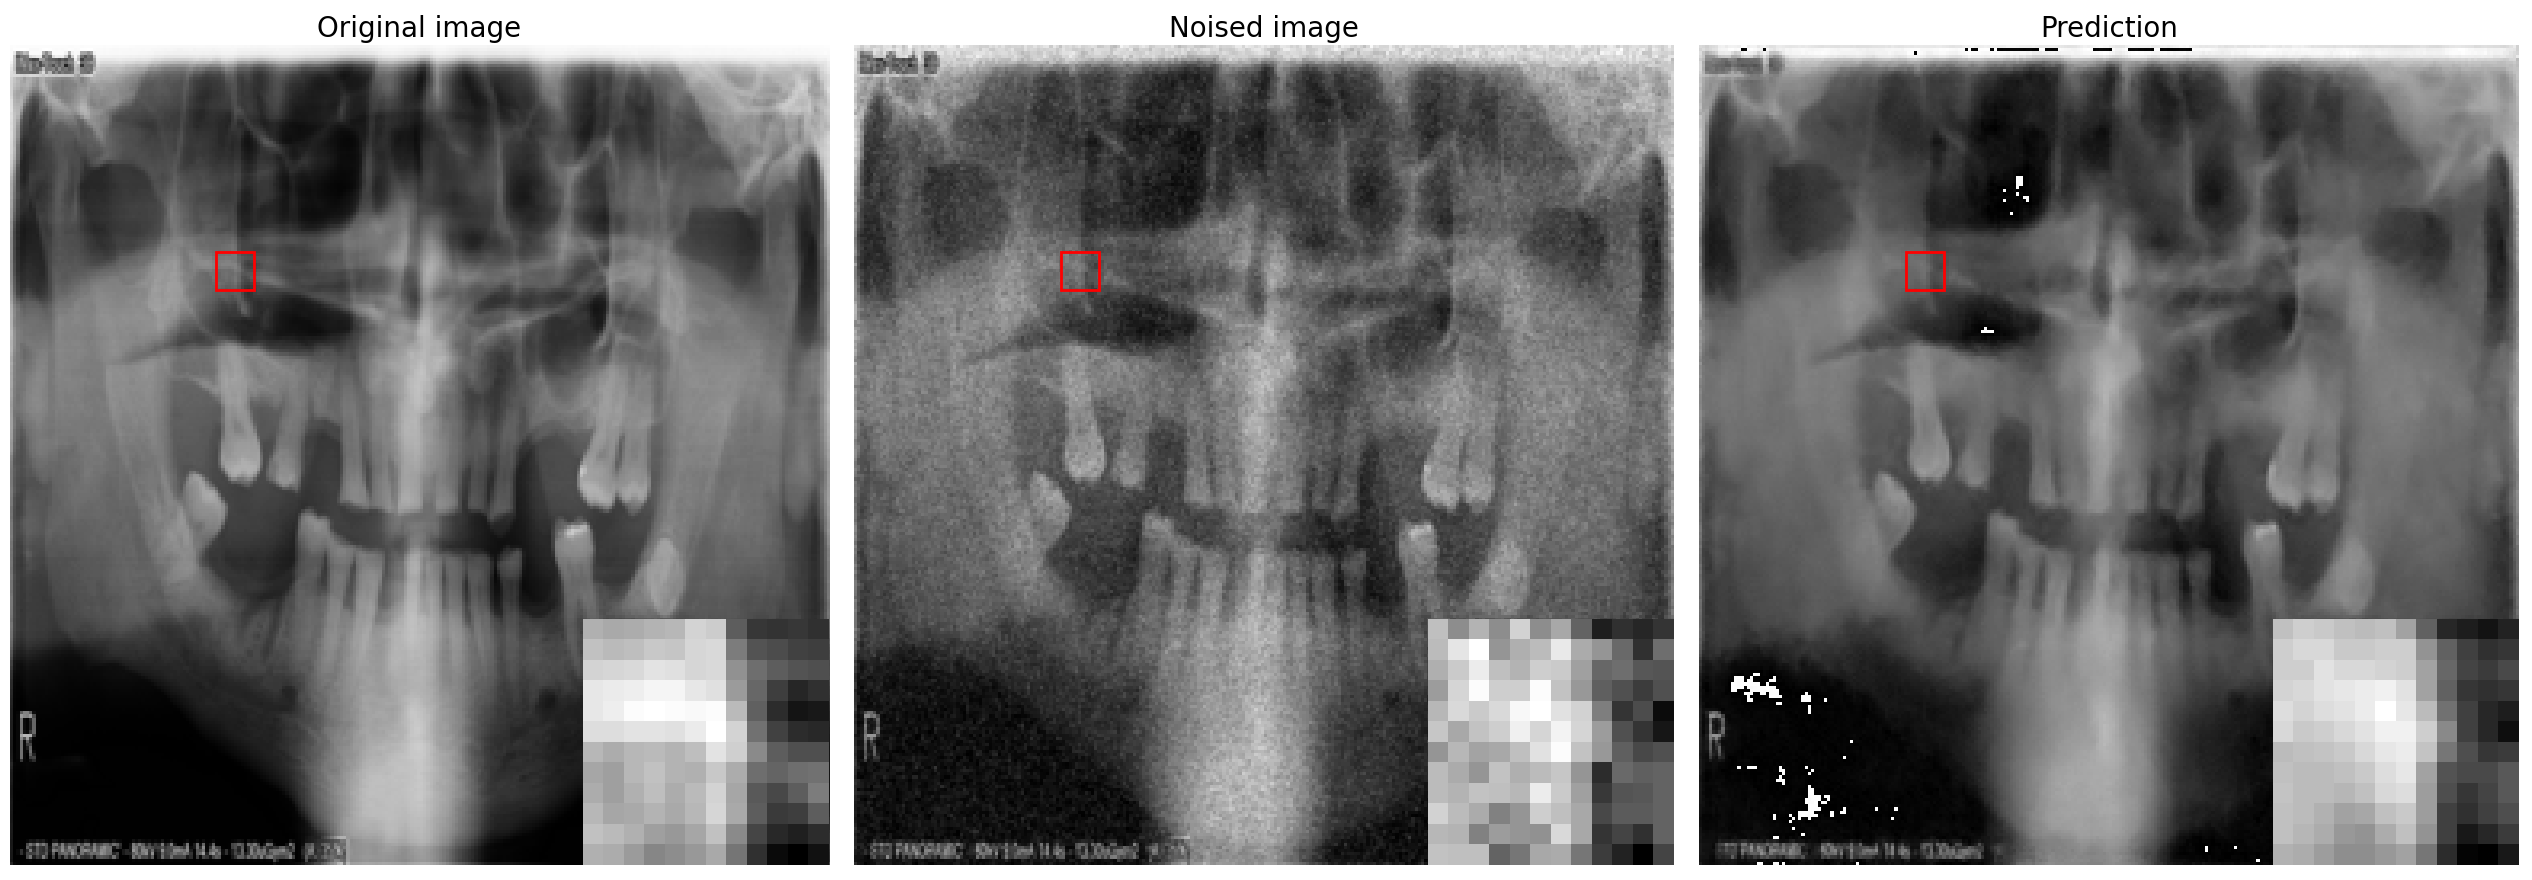
\includegraphics[width=\linewidth]{Prilohy/Obrazky/DnCNN_teeth.png}
    \caption{Ukázka odstranění šumu ze snímku zubů pomocí DnCNN}
    \label{fig:DnCNN_teeth}
\end{figure}

\begin{table}[h]
    \centering
    \begin{tabular}{|l|l|l|}
    \hline
    \textbf{Typ šumu}               & \textbf{PSNR} & \textbf{SSIM} \\ \hline
    Poissonův                       & 36 dB         &  97 \%        \\ \hline
    Speckle                         & 34 dB         &  93 \%        \\ \hline
    Sůl a pepř                      & 29 dB         &  85 \%        \\ \hline
    Poissonův, speckle              & 33 dB         &  92 \%        \\ \hline
    Poissonův, sůl a pepř           & 29 dB         &  85 \%        \\ \hline
    Speckle, sůl a pepř             & 28 dB         &  83 \%        \\ \hline
    Poissonův, speckle, sůl a pepř  & 28 dB         &  83 \%        \\ \hline
    \end{tabular}
    \caption{Ukázka výsledků kvalitu obrazu po odšumění pomocí ensemble averaging}
    \label{tab:DnCNNResults}
\end{table}

\subsection{Vyhodnocení natrénovaných modelů sítě DAE}
Následně byla hodnocena výkonnost autoenkodér pro redukci šumu (DAE), což je složitý model s přibližně 10 miliony parametry. Než jsem dospěl k nejlepšímu modelu, bylo nutné vytvořit několik variant základní architektury DAE. Nejdříve jsem zkoušel jednoduchou síť s pár vrstvami bez použití skip connections. Tento model ovšem nebyl úspěšný. Další model byl navržen v podobném duchu jako DnCNN a jeho úkolem bylo detekovat šum, nikoli tvořit nový odšuměný snímek. To se ovšem ukázalo jako liché a tento přístup také nebyl úspěšný. Nejlepší model byl natrénován pomocí architektury nastíněné výše s využitím augmentačních technik popsaných v tabulce \ref{tab:DAE_augmentation}. Přes svůj potenciál architektura DAE nedosáhla tak dobrých výsledků jako DnCNN. Tento suboptimální výkon je přičítán složitosti modelu a omezenému množství tréninkových dat, což vedlo k přeučení po zhruba 30 epochách u nejlepšího modelu. DAE dosáhl průměrného PSNR kolem 23 dB, což znamená sníženou účinnost při odstraňování šumu ve srovnání s DnCNN. Nicméně hodnota SSIM pro DAE byla 80 \%, což je hodnota nižší v porovnání s DnCNN, stále ale představuje přiměřenou strukturální podobnost. Jako v případě předešlých vyhodnocení jsou výsledky pro jednotlivé typy šumů zobrazeny v následující tabulce \ref{tab:DAEResults}. Výsledky ukazují, že u mnoha typů šumů došlo v metrice PSNR ke zhoršení, ale metrika SSIM vykazuje pro každý typ šumu vyšší hodnotu než v případě zašuměných snímků. To poukazuje na fakt, že snímky byly vylepšeny, ale jelikož autoenkodér snímek vytváří, tak mohlo dojít ke ztrátě některých informací.

\begin{table}[h]
    \centering
    \begin{tabular}{|l|l|l|}
    \hline
    \textbf{Augmentace}  & \textbf{Popis}                          & \textbf{Pravděpodobnost} \\ \hline
    Gaussovský blur      & Aplikuje Gaussovské rozostření.         &  20 \%                   \\ \hline
    Ostrost obrazu       & Upravuje ostrost obrazu.                &  20 \%                   \\ \hline
    Autokontrast         & Automaticky vyrovnává kontrast snímků.  &  30 \%                   \\ \hline
    Ekvalizace           & Ekvalizace histogramu.                  &  40 \%                   \\ \hline
    Horizontální otočení & Horizontální překlopení snímku.         &  50 \%                   \\ \hline
    \end{tabular}
    \caption{Přehled augmentací aplikovaných při učení DAE}
    \label{tab:DAE_augmentation}
\end{table}

\begin{table}[h]
    \centering
    \begin{tabular}{|l|l|l|}
    \hline
    \textbf{Typ šumu}               & \textbf{PSNR} & \textbf{SSIM} \\ \hline
    Poissonův                       & 26 dB         &  87 \%        \\ \hline
    Speckle                         & 26 dB         &  85 \%        \\ \hline
    Sůl a pepř                      & 23 dB         &  82 \%        \\ \hline
    Poissonův, speckle              & 25 dB         &  85 \%        \\ \hline
    Poissonův, sůl a pepř           & 23 dB         &  82 \%        \\ \hline
    Speckle, sůl a pepř             & 23 dB         &  80 \%        \\ \hline
    Poissonův, speckle, sůl a pepř  & 23 dB         &  80 \%        \\ \hline
    \end{tabular}
    \caption{Ukázka výsledků kvalitu obrazu po odšumění pomocí ensemble averaging}
    \label{tab:DAEResults}
\end{table}

\section{Aplikace implementovaných metod a měření vlivu předzpracování na efektivitu segmentačních modelů}
V této sekci se zaměřím na měření vlivu předzpracování na efektivitu segmentačních modelů. Při popisování struktury projektu již zazněl název architektury, na které bude vliv předzpracování měřen. Jedná se o široce používanou architekturu v oblasti segmentace medicínských dat, nesoucí název U-Net. Podrobné informace o architektuře sítě U-Net lze nalézt v článku Ronnebergera a kol. (2015) \cite{UNET_paper}.

Segmentační modely sítě U-Net jsem trénoval na několika datových sadách. Nejdříve jsem natrénoval a změřil výkon modelu na originálních nezašuměných datech. Tento model sloužil pro porovnání vlivu předzpracování a jednalo se o vrchol možného zlepšení dalších modelů. Dále jsem použil pro trénování datovou sadu zašuměných snímků, která představovala pravý opak prvního natrénovaného modelu. Jinými slovy mělo jít o nejhorší model, který jsem se poté snažil vylepšit pomocí technik pro předzpracování snímků. Abych mohl trénovat modely využívající metody předzpracování, tak jsem vytvořil celkem šest datových sad, rozdělených po dvojicích. Každá první datová sada z dvojice zahrnovala snímky plic a druhá snímky zubů upravených pomocí sítě DnCNN, DAE a ensemble averaging techniky.

Před samotným měřením vlivu předzpracování na segmentační modely, je důležité pochopit, jak různé přístupy k předzpracování ovlivňují kvalitu segmentace při různých problémech. Jak již bylo popsáno v sekci zaměřené na popis datových sad, je pro tento účel nutné rozlišovat mezi jednoduššími a složitějšími úlohami segmentace. Proto jsou v následujících podsekcích uvedeny výsledky měření pro dvě odlišné úlohy: binární segmentace rentgenových snímků plic a vícetřídní segmentace rentgenových snímků zubů. Tato rozdělení umožňují detailně posoudit efektivitu jednotlivých metod předzpracování v různých kontextech.

\subsection{Měření vlivu předzpracování obrazu na binární segmentaci rentgenových snímků plic}
Pro měření vlivu předzpracování dat bylo trénováno několik různých kombinací modelů, které měly odhalit, zda a jaký má předzpracování dopad na průběh trénování a výkon jednotlivých modelů. Modelů bylo trénováno několik s odlišnými hyperparametry a s aplikací augmentačních technik. Už u prvních modelů bylo patrné, že úloha segmentace plic není obtížná a architektura U-Net si dokáže poradit se znehodnocenými snímky s přidaným šumem. I doba učení se téměř neměnila a všechny učené modely byly dotrénovány přibližně kolem 30 epochy. 

Navzdory různým nastavením hyperparametrů a aplikaci augmentačních technik vykazovaly všechny modely známky přeučení přibližně po zmíněných 30 epochách. To naznačuje, že problém binární segmentace snímků plic je relativně jednoduchý a model U-Net je schopen detekovat okraje plic a jejich tvar i přes vrstvu šumu bez potřeby intenzivního předzpracování.

Níže je uvedena tabulka \ref{tab:BinaryUnetResults}, která zobrazuje výsledky pěti nejlépe natrénovaných modelů, včetně jejich dosažených hodnot Jaccard indexu:

\begin{table}[h]
    \centering
    \begin{tabular}{|l|c|}
        \hline
        \textbf{Model}                            & \textbf{Jaccard Index} \\ \hline
        U-Net (Originální snímky)                 & 90.2 \%                 \\ \hline
        U-Net (Předzpracování Ensemble Averaging) & 89.7 \%                 \\ \hline
        U-Net (Předzpracování DnCNN)              & 89.5 \%                 \\ \hline
        U-Net (Předzpracování DAE)                & 89.3 \%                 \\ \hline
        U-Net (Zašuměná data)                     & 87.5 \%                 \\ \hline
    \end{tabular}
    \caption{Výsledky nejlepších modelů U-Net pro binární segmentaci rentgenových snímků plic.}
    \label{tab:BinaryUnetResults}
\end{table}

Tato tabulka ukazuje, že i model trénovaný na zašuměných datech dosáhl Jaccard indexu blízkého 90 \%, což potvrzuje hypotézu, že tato segmentační úloha je natolik jednoduchá, že model U-Net je schopen efektivně detekovat okraje plic i bez výrazného vlivu předzpracování dat. Tento výsledek podtrhuje robustnost a schopnost U-Net architektury vyrovnat se s jednoduchými segmentačními úlohami i za podmínek přítomnosti šumu.

\begin{figure}[h]
    \centering
    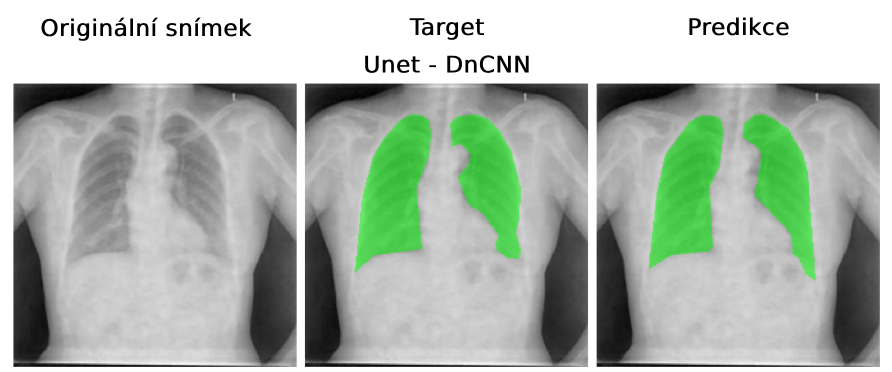
\includegraphics[width=\linewidth]{Prilohy/Obrazky/BinaryUnetDnCNN.png}
    \caption{Ukázka segmentace plic pomocí modelu sítě U-Net na snímku předzpracovaném sítí DnCNN (ukázka predikcí všech modelů je k dispozici na GitHubu této práce).}
    \label{fig:BinaryUnet}
\end{figure}

\subsection{Měření vlivu předzpracování obrazu na vícetřídní segmentaci rentgenových snímků zubů}
Měření vlivu předzpracování obrazu v předchozí části přineslo velmi zajímavé výsledky. Tato podsekce se zaměří na mnohem komplexnější problém, konkrétně vícetřídní klasifikaci 32 zubů, na které by se vliv předzpracování mohl projevit mnohem znatelněji.

Stejně jako v předešlé části bylo trénováno několik variant modelů, počínaje modelem trénovaným na originálních datech, modelem trénovaným na zašuměných datech a modelech využívajících odšuměná data. Nejlepší model U-Net dosáhl na originálních snímcích pouze 65 \% Jaccard indexu, což jasně značí rozdíl náročnosti segmentace této úlohy na rozdíl od snímků plic. Na zašuměných snímcích byla hodnota Jaccard indexu mnohem nižší, konkrétně 55 \%. Z výsledku je patrné, že šum velmi ztížil modelu schopnost rozpoznat zuby ve snímku a správně je segmentovat.

Výsledky technik pro předzpracování byly velmi zajímavé. Předzpracování pomocí modelu architektury DnCNN dosáhlo Jaccard indexu přibližně 64 \%, což je srovnatelné s výsledky na originálních snímcích. Je tedy vidět, že předzpracování obrazu má znatelný dopad na schopnost sítě U-Net segmentovat objekty. Model, využívající snímky předzpracované pomocí DAE dosáhl Jaccard indexu pouhých 58 \%, což je mírné zlepšení oproti zašuměným snímkům, avšak nižší v porovnání s DnCNN. Pravděpodobně tato složitější architektura nebyla vystavena dostatečnému množství trénovacích dat. Nejlepších výsledků bylo dosaženo pomocí techniky ensemble averaging, která dosáhla Jaccard indexu 65 \%. Tento výsledek je pozoruhodný, neboť překonal nejlepší model trénovaný na originálních snímcích. Tento výsledek by mohl naznačovat, že metody pro předzpracování snímků použité v ensemble averaging by mohly nejen odstranit šum přidaný do snímků uměle, ale také mohly zlepšit kvalitu samotných originálních snímků. Výsledný rozdíl je ale velmi nepatrný a jelikož je učení modelů nedeterministické, nejspíše se jedná pouze o náhodu. Ukázka učení modelů vícetřídní segmentace je zobrazena v grafu \ref{fig:MulticlassUnet_plot}.

\begin{figure}[h]
    \centering
    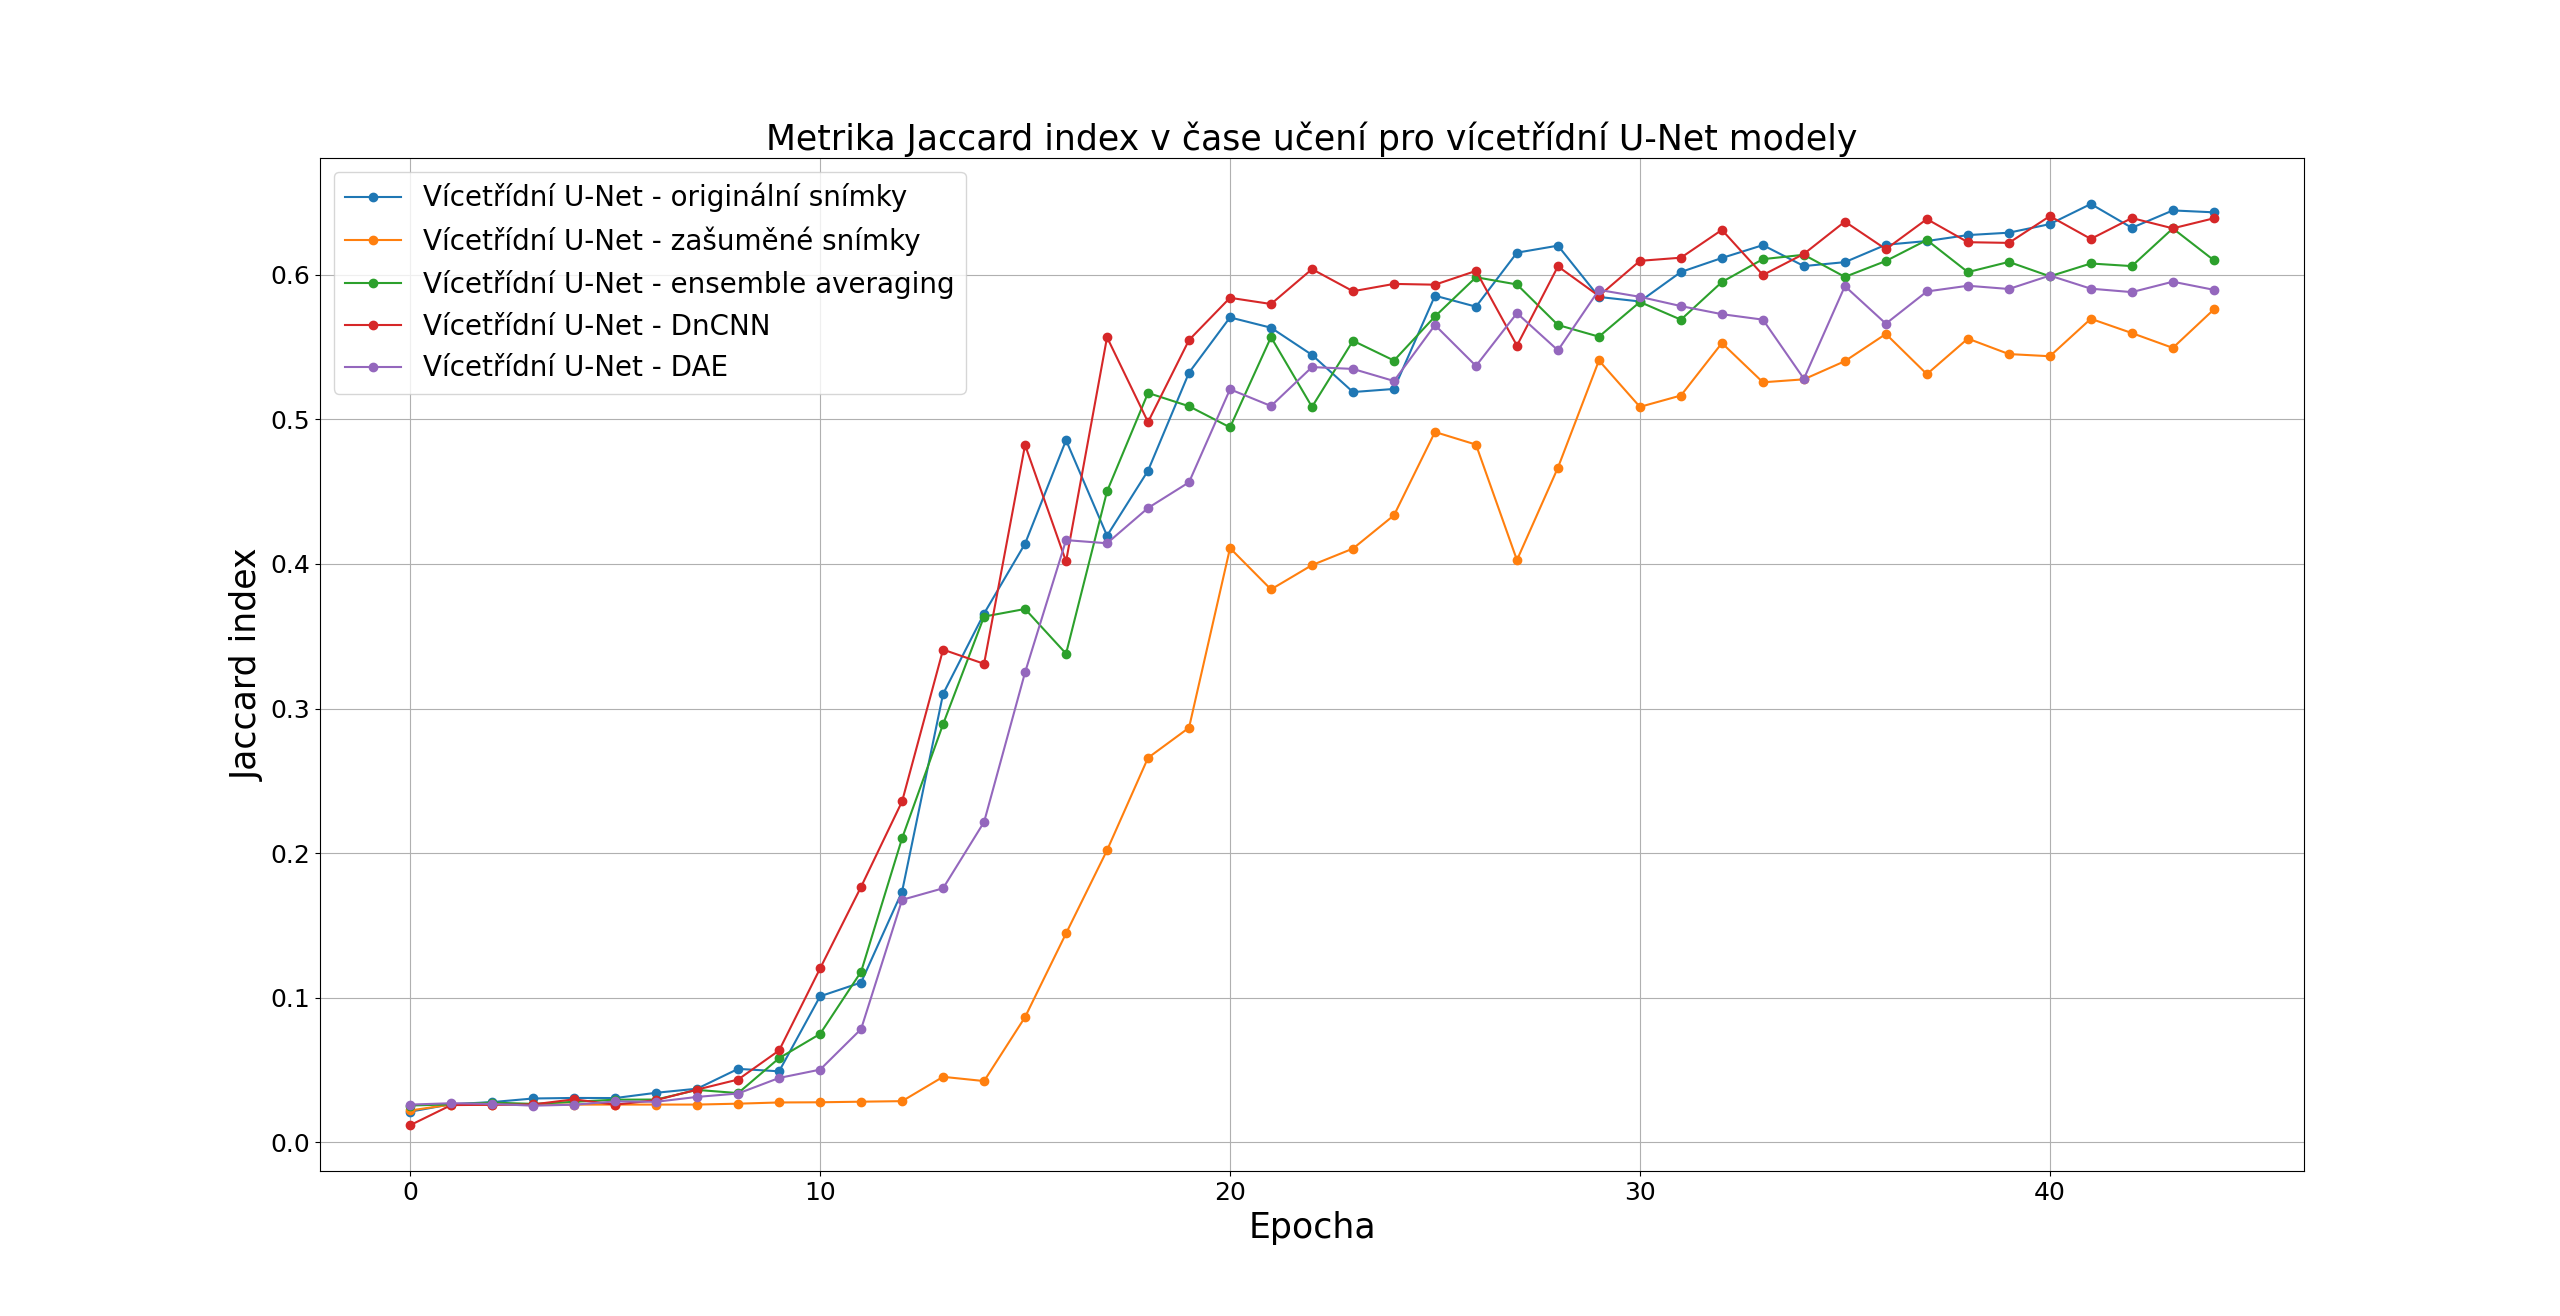
\includegraphics[width=\linewidth]{Prilohy/Obrazky/Jaccard_index_multiclass_unet.png}
    \caption{Graf zobrazující průběh učení modelů vícetřídní segmentace. Z grafu je patrné, že učení na zašuměných datech bylo náročnější v porovnání s ostatními modely.}
    \label{fig:MulticlassUnet_plot}
\end{figure}

V průběhu experimentů byly rovněž aplikovány různé techniky augmentace dat, které měly za cíl zvýšit rozmanitost trénovací sady a zlepšit schopnost modelů generalizovat. Nicméně, augmentace dat měly pouze minimální dopad na výkonnost a správnost predikcí, přinášející zlepšení přibližně o 1 \% Jaccard indexu.

Níže je uvedena tabulka \ref{tab:MulticlassUnetResults}, která zobrazuje výsledky pěti nejlépe natrénovaných modelů:

\begin{table}[h]
    \centering
    \begin{tabular}{|l|c|}
        \hline
        \textbf{Model}                            & \textbf{Jaccard Index} \\ \hline
        U-Net (Předzpracování Ensemble Averaging) & 65.5 \%                 \\ \hline
        U-Net (Originální snímky)                 & 65.2 \%                 \\ \hline
        U-Net (Předzpracování DnCNN)              & 64.8 \%                 \\ \hline
        U-Net (Předzpracování DAE)                & 58.3 \%                 \\ \hline
        U-Net (Zašuměná data)                     & 55.4 \%                 \\ \hline
    \end{tabular}
    \caption{Výsledky nejlepších modelů U-Net pro binární segmentaci rentgenových snímků plic.}
    \label{tab:MulticlassUnetResults}
\end{table}

Z tabulky je patrné, že předzpracování vhodnou metodou má výrazný vliv na výkon modelů pro segmentaci zubů. Tyto výsledky naznačují, že u složitějších úloh může být předzpracování přínosné a může zlepšit výkonnost trénovaných modelů.

\begin{figure}[h]
    \centering
    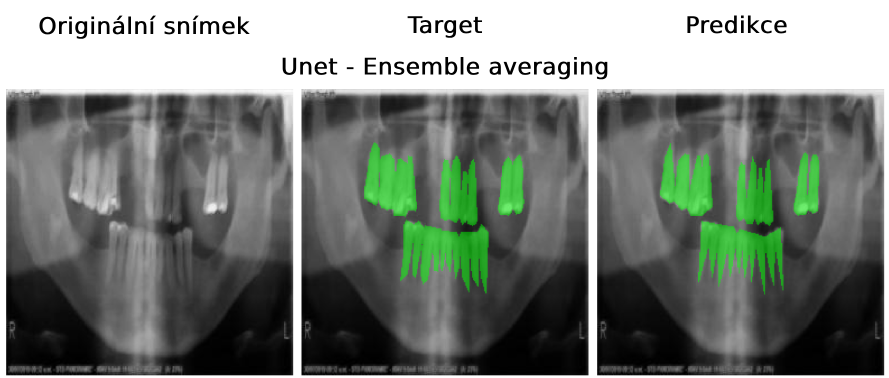
\includegraphics[width=\linewidth]{Prilohy/Obrazky/MulticlassUnetEnsemble.png}
    \caption{Ukázka segmentace zubů pomocí modelu sítě U-Net na snímku předzpracovaném metodou ensemble averaging.}
    \label{fig:MulticlassUnet}
\end{figure}

\chapter{Zhodnocení} 
Segmentace snímků plic pomocí binárních modelů sítě U-Net odhalila, že síť je schopná naučit se segmentovat rentgenové snímky i za přítomnosti šumu. Jelikož jsou v těchto snímcích dobře viditelné hrany plic a jejich plochy jsou velké a příliš nemění tvar, předzpracování obrazu přineslo pouze minimální, skoro mizivé zlepšení výkonu modelů. Modely sítě U-Net dosáhly vysokého skóre Jaccard Index napříč různými modely, včetně těch, které byly trénovány na zašuměných snímcích. To naznačuje, že pro jednoduché úkoly, jako je segmentace plic, mohou stačit pouze jednoduché techniky předběžného zpracování, jako je ekvalizace histogramu, úprava kontrastu a další jiné základní vylepšení obrazu. Tyto metody dokážou připravit snímky adekvátně bez potřeby složitých algoritmů pro redukci šumu.

Segmentace snímků zubů představovala zajímavější a náročnější problém. Složitost rozlišení a segmentace 32 různých zubů v rentgenových snímcích znamenala, že předběžné zpracování mělo výraznější dopad na kvalitu obrazu a výkon modelů. Výsledky poukázaly na několik klíčových zjištění. Složité sítě nejsou vždy nejlepším řešením. Příkladem je autoenkodér pro redukci šumu (DAE), který navzdory své složitosti nevykazoval dobré výsledky. Nejlepší model s Jaccard indexem 58 \% ukázal, že takto složité architektury mohou vyžadovat podstatně větší datovou sadu, aby se správně naučili snímky segmentovat.

Další zjištění spočívalo v použití metody ensemble averaging. Očekávalo se, že tato metoda nebude dostatečně silným nástrojem pro redukci šumu z důvodu zaměření jednotlivých filtrů na konkrétní typy šumu. Výsledek odšumění pomocí této metody byl velmi překvapivý, neboť metoda dokázala konkurovat neuronovým sítím a v některých případech vykazovala nejlepší výsledky při předzpracování rentgenových snímků zubů. To naznačuje, že i základní metody předzpracování mohou účinně redukovat šum a tím zlepšit kvalitu obrazu. Úspěch těchto jednoduchých filtrů naznačuje, že mohou hrát zásadní roli při zlepšování kvality obrazu bez výpočetní režie složitějších metod. 

V neposlední řadě je nutné podotknout, že výkon architektury U-Net při segmentaci zubů byl výrazně horší ve srovnání se segmentací plic. To může ukazovat na fakt, že tato architektura není dostatečná pro úlohu tohoto rozsahu nebo na příliš malou datovou sadu, která nezahrnovala všechna specifika zubů.

\chapter{Závěr}
Hlavním cílem této diplomové práce bylo zjistit jaký vliv má předzpracování obrazu a augmentace dat na segmentaci rentgenových snímků. Předmětem zkoumání bylo měření vlivu technik založených na standardních metodách a také modelech využívajících neuronové sítě v závislosti na míře ovlivnění výkonu modelů architektury U-Net pro segmentaci obrazu.

V úvodní části práce byla pozornost věnována primárně vybraným standardním algoritmům, vylepšující obraz a redukující šum, se zaměřením na základní principy jejich fungování. V návaznosti se práce zaměřila na představení základního přehledu neuronových sítí, využívaných zejména pro práci s obrazovými daty, podrobně byly popsány jejich hlavní komponenty, struktura a funkčnost. V neposlední řadě byly vylíčeny techniky augmentace dat, které zvyšují rozmanitost tréninkových sad a podporují lepší generalizaci modelů.

Začátek druhé kapitoly byl zaměřen na popis dvou vybraných datových sad, které obsahovaly rentgenové snímky plic a panoramatické snímky zubů. Zmíněné datové sady reprezentovaly dvě úrovně složitosti problémů, aby bylo možné důkladně prozkoumat vliv předzpracování dat, a zda je neuronová síť U-Net schopna adaptovat se na degradovaná obrazová data. Na rentgenové snímky z datových sad byly aplikovány tři druhy nejčastěji se vyskytujících šumů v rentgenových snímcích samostatně nebo v kombinaci. Z popsaných standardních metod byly následně vybrány ty, které se ukázaly jako nejúčinnější při redukci šumu ve vytvořených datech a byla z nich vytvořena metoda zvaná \textit{ensemble averaging}. Zvláštní pozornost byla věnována implementaci vybraných architektur neuronových sítí pro redukci šumu, jako je autoenkodér pro redukci šumu (\textit{DAE}) a konvoluční neuronová síť pro redukci šumu (\textit{DnCNN}), jenž se staly hlavním bodem zájmu při zlepšování kvality obrazových dat.

V poslední části práce byl měřen vliv předzpracování dat na výkonnost modelů neuronové sítě U-Net pro segmentaci obrazu. Nejprve byly provedeny experimenty s binární segmentací rentgenových snímků plic, které sloužily pro zjištění, zda je nutné používat techniky předzpracování i pro snadné úlohy segmentace. Poté se práce zaměřila na složitější úlohu segmentace zubů, kde obtížnost nespočívala pouze v ohodnocení samotných zubů, ale také v menší velikosti datové sady. Na této úloze bylo jasně znatelné zlepšení v případě použití technik pro předzpracování obrazu, avšak augmentace dat přispěla k výkonnosti modelů jen mírně. Výsledky naznačily, že pro takto složité úlohy je potřeba jak kvalitní předzpracování dat, tak i dostatečně velká a rozmanitá datová sada.

Celkově tato práce ukázala, že účinnost předzpracování a augmentace dat závisí na složitosti zadané úlohy, schopnosti dané architektury a velikosti datové sady. V případě složitých úloh či nedostatku některého ze zmíněných faktorů může předzpracování obrazu zlepšit výkonnost segmentačních modelů. Tyto poznatky přispívají k lepšímu porozumění role předzpracování a augmentace dat v oblasti segmentace rentgenových snímků a poskytují základ pro další výzkum a praktické aplikace v této oblasti.

\printbibliography[title=Seznam použitých zdrojů]

\listoffigures

\listoftables

\lstlistoflistings

\appendix

\chapter{Externí přílohy\label{sec:ep}}

%Na úložiští GitHub mohou byt uloženy tyto externí přílohy:

%\begin{itemize}
%\item \textbf{zdrojové kódy}
%\item \textbf{doplňkové texty} (například jak instalovat aplikaci, manuály aplikace)
%\item \textbf{schémata} (především, pokud se nevejdou na stranu A4 a jejich vytištění je tak problematické)
%\item \textbf{screenshoty} (v textu práce lze použít jen omezený počet snímků obrazovky, které navíc nemusí být při černobílém tisku příliš %přehledné)
%\item \textbf{videa} (například ovládání aplikace)
%\end{itemize}

%V každém případě by to však měli být pouze materiály, které jste vytvořili sami. Materiály jiných autorů uvádějte v seznamu použité %literatury (včetně případných odkazů na jejich originální umístění).

%V této kapitole stačí uvést pouze základní strukturu úložiště (co se kde nalézá a jakou má funkci) například v podobě tabulky. 

Externí přílohy této diplomové práce jsou umístěny na adrese: \\
\url{https://github.com/Cemonix/Impact-of-Preprocessing}

Struktura repozitáře je následující:
\begin{longtable}{ll}
\hline
main.py & Hlavní skript, obsahující všechny funkce pro trénování, testování a tvorbu datasetů \\
common & Skripty pro vizualizaci, tvorbu datasetů a základní struktury tříd \\
configs & Konfigurační soubory pro různé experimenty a nastavení filtrů \\
preprocessing & Předzpracování dat pomocí standardních metod a neuronových sítí \\
unet & Implementace U-Net modelu a související skripty \\
statistics\_methods & Složka, zahrnující skripty pro statistické metody \\
results & Snímky s výsledky a ukázkami predikcí \\
\hline
\end{longtable}

%Všechny tyto soubory jsou potřeba pro překlad dokumentu (logo stačí jedno v příslušné jazykové verzi).

\end{document}
